\documentclass[aps, secnumarabic, balancelastpage, asmath, amssymb, nofootinbib, floatfix,]{revtex4-2}
\usepackage{minted}
\usepackage{graphicx}
\usepackage{float}
\usepackage{caption}
\usepackage{siunitx}
\usepackage[export]{adjustbox}
\usepackage{subcaption}
\usepackage{amsmath}
\usepackage{hyperref}
\usepackage{subcaption}
\usepackage{tikz}
\usepackage{multirow}
% \usepackage[table,xcdraw]{xcolor}
\usepackage{xcolor}
\usepackage{cprotect}
\usepackage{verbatimbox}
\usepackage{listings}
\usepackage{xparse}
\usepackage{listings}
%\usepackage{times}
\NewDocumentCommand{\codeword}{v}{%
\texttt{\textcolor{black}{#1}}%
}

\hypersetup{colorlinks=true, pdfstartview=FitV, linkcolor=blue, citecolor=black, plainpages=false, pdfpagelabels=true, urlcolor=blue}

\newenvironment{code}{\captionsetup{type=listing}}{}
% \SetupFloatingEnvironment{listing}{name=Source Code}

\definecolor{backcolour}{rgb}{0.95,0.95,0.92}
\definecolor{mGreen}{rgb}{0,0.6,0}
\definecolor{mGray}{rgb}{0.5,0.5,0.5}
\definecolor{mPurple}{rgb}{0.58,0,0.82}
\definecolor{backgroundColour}{rgb}{0.95,0.95,0.92}
\definecolor{LightGray}{gray}{0.9}

\setlength{\arrayrulewidth}{0.3mm}
\setlength{\tabcolsep}{5pt}
\renewcommand{\arraystretch}{1.5}
\graphicspath{{./image/}}

\usepackage{setspace}
\usepackage{titletoc}
%\contentsmargin{2.55em}
\dottedcontents{chapter}[1.5em]{}{2.3em}{1pc}
\dottedcontents{section}[1.5em]{}{1.7em}{0.5pc}
\dottedcontents{subsection}[3.9em]{}{2.4em}{0.5pc}
\dottedcontents{subsubsection}[6.6em]{}{2.7em}{0.5pc}
\dottedcontents{paragraph}[9.5em]{}{1.9em}{0.5pc}

\usepackage{etoolbox}
\makeatletter
\pretocmd{\chapter}{addtocontents{toc}{\protect\addvspace{15\p@}}}{}{}
\pretocmd{\section}{\addtocontents{toc}{\protect\addvspace{9\p@}}}{}{}
%\pretocmd{\subsection}{\addtocontents{toc}{\protect\addvspace{15\p@}}}{}{}
\makeatother


\stepcounter{secnumdepth}
\stepcounter{tocdepth}

% Usual (decimal) numbering
\renewcommand{\thesection}{\arabic{section}}
\renewcommand{\thesubsection}{\thesection.\arabic{subsection}}
\renewcommand{\thesubsubsection}{\thesubsection.\arabic{subsubsection}}

% Fix references
\makeatletter
\renewcommand{\p@subsection}{}
\renewcommand{\p@subsubsection}{}
\makeatother

\lstset
{ %Formatting for code in appendix
    basicstyle=\footnotesize,
    numbers=left,
    stepnumber=1,
    showstringspaces=false,
    tabsize=1,
    breaklines=true,
    breakatwhitespace=false,
    %basicstyle=\ttfamily,
    %columns=fullflexible,
    frame=single,
    postbreak=\mbox{\textcolor{red}{$\hookrightarrow$}\space},
    numbersep=5pt,
}

\usepackage{wrapfig}

\begin{document}
%top matter
    \begin{titlepage}
   \begin{center}
       \vspace*{1cm}

	\Huge
       \textbf{CE339 - High Level Digital Design}

       \vspace{0.5cm}
       
       \LARGE
        \textbf{Assignment 2 -- ``Snake'' Video Game}
            
       \vspace{1.5cm}

       \textbf{Akshay Gopinath}\\
       \textbf{Registration Number: 2005614}\\
       \textbf{Word Count: 3944}\\

       \vfill
        \begin{figure}[h]
        
        
\includegraphics[scale = 0.85]{University}
        
   	\end{figure}
        \vfill
            
       A report presented for the degree of\\
       Electronic Engineering
            
       \vspace{1cm}
     
            
       School of Computer Science and Electronic Engineering\\
       University of Essex\\
       England\\
       \today

   \end{center}
\end{titlepage}

%\thispagestyle{plain}
%\Large
%\textbf{Contributions}

%\clearpage

\thispagestyle{plain}
\begin{center}
    \Large
    \textbf{CE339 - High Level Digital Design}
        
    \vspace{0.4cm}
    \large
    \textbf{Assignment 2 -- ``Snake'' Video Game}
        
    \vspace{0.4cm}
    \textbf{Akshay Gopinath}
       
    %\vspace{0.9cm}
    \section*{Abstract}
    \fontsize{11pt}{12pt}\selectfont
    
\end{center}
\fontsize{11pt}{12pt}\selectfont
{
\setlength{\parindent}{0pt}


This report aims to showcase and explain the design as well the process of developing a complex digital system. The digital system designed in this experiment is a simplified version of the classic `snake' game. The main aim is to design a playable snake game with hardware sprites (static and animated), whilst showing the player score. The target board is the Digilent Basys3, hence the VGA port is used to display graphics and the 7-segment display is used to show the score.

}

\clearpage

\thispagestyle{plain}
\begin{center}
    \Large
    \textbf{CE339 - High Level Digital Design}
        
    \vspace{0.4cm}
    \large
    \textbf{Assignment 2 -- ``Snake'' Video Game}
        
    \vspace{0.4cm}
    \textbf{Akshay Gopinath}
       
    %\vspace{0.9cm}
    \section*{Acknowledgements}
    \fontsize{11pt}{12pt}\selectfont
    
\end{center}
\fontsize{11pt}{12pt}\selectfont
{
\setlength{\parindent}{0pt}

I would like to give my deepest appreciation to those who provided me the possibility to complete my this
design challenge. A special gratitude I give to the module supervisor of the CE339 module, Dr. Wenqiang Yi for their guidance and encouragement, and providing me with the necessary material to learn how to complete this project.

I would also like to acknowledge with appreciation, the help of the technicians from Laboratory 8, who provided
me access to the necessary equipment to complete the project, both during and outside lab sessions hours. A very
special thanks goes to my peer, PhD student and GLA, Michal Borowski who provided me with tips and guidance to complete my design, especially when it came to rendering hardware sprites on the VGA display.

}

\clearpage

\tableofcontents

\clearpage

\listoffigures
\clearpage

% \listoftables

\clearpage


\section{\fontsize{11.3pt}{12pt}\selectfont \bf Introduction}
\fontsize{11pt}{12pt}\selectfont
\label{sec:1}

{
\setlength{\parindent}{0pt}

This report documents an experiment to design a ``Snake'' Video Game on hardware using a Hardware Description Language (HDL) called VHDL (Very High Speed Integrated Circuit Hardware Design Language). The target platform is the Digilent Basys3 Board which houses an Artix-7 based FPGA[1]. The VHDL code is synthesised using Xilinx Vivado. The VGA (Video Graphics Array) port on the Basys3 board is used to display the game on a compatible monitor and the player score is shown on the 7-segment display. This report will explain the design in a top-down approach, whilst going into detail on every sub-components. The top level schematic will generate the necessary signals required to correctly display the game and the score, such as the VGA synchronisation signals, RGB (red, green, blue) colour signals and the 7-segment display cathode and anode signals.

\section{\fontsize{11.3pt}{12pt}\selectfont \bf The Design}

\subsection{\fontsize{11.4pt}{12pt}\selectfont \bf High Level Overview \label{sec:2.1}}

\fontsize{11pt}{12pt}\selectfont
\label{sec:2}

\begin{figure}[h]
  \centering
  %\captionsetup{justification=centering}
  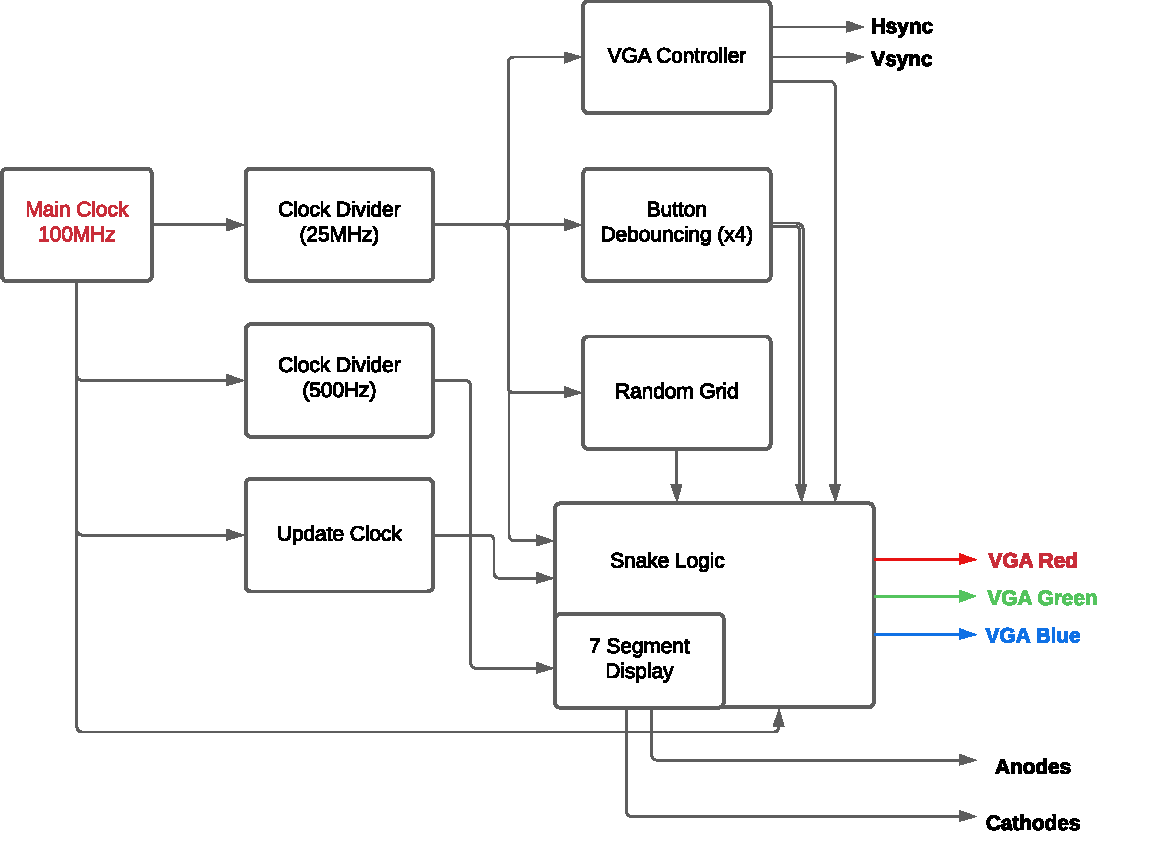
\includegraphics[scale = 0.7]{VGA-Flow - Page 1.pdf}
  \caption{\em High level architecture of the system}
  \label{fig:1}
\end{figure}

Figure \ref{fig:1} above shows the high level block diagram of the system. The main clock is from the Basys3 board which is at 100MHz frequency. The targer resolution is 640x480. The pixel clock is 25MHz, with a refresh rate of 60Hz. In order to generate the required synchronisation signals (by the VGA Controller module) for these specifications, the VGA controller module needs a 25MHz a clock. Hence the 100MHz master clock is given as input to a clock divider to generate this frequency. The 25MHz clock is also used for button debouncing (to keep it in synchronisation with the graphics being rendered to the screen), and also for the Random Grid module. Another clock divider was instantiated to generate a 500Hz clock. The 500Hz clock is used for the time multiplexed 7-segment display driver, which resides inside the Snake Logic module. The update clock is a module used to generate a pulse at a desired frequency (in this case 25Hz), which is high only for one clock cycle of the master clock. The purpose of this module is to set the update frequency of the game logic, hence the output of the update clock is given as input to the Snake Logic module. The Random Grid module is used to generate pseudo random locations for the positions of the food in the game. And the output is given to the Snake Module as input. The VGA Controller module generates the horizontal and vertical synchronisation signals for the VGA Port. It also outputs the current x and y count co-ordinate as well as the blanking signal for the Snake Logic module to keep track of the screen position. The Snake Logic block is the main heart of the system. The Snake Logic module is the heart of the entire system, and contains the game main logic, as well as the rendering signals. This module contains many processes to control game elements such as the snake location direction, snake direction, snake size, game state, game levels etc. The module also contains the 7-segment display driver and BCD (Binary Coded Decimal) counters to display the score whilst playing the game. This module outputs the anode and cathode signals for the 7-segment display as well as the red, green and blue signals for the VGA port. The high level diagram from Figure \ref{fig:1} represents the main top level file shown in \hyperref[code:main]{Source Code 1}.

\vspace{-1.0em}
\subsection{\fontsize{11.4pt}{12pt}\selectfont \bf Detailed Overview \label{sec:2.2}}

\subsubsection{\fontsize{10pt}{12pt}\selectfont \bf snake \label{sec:2.2.1}}

\vspace{-1.5em}
\begin{wrapfigure}[14]{l}{0.6\textwidth}
    \centering
    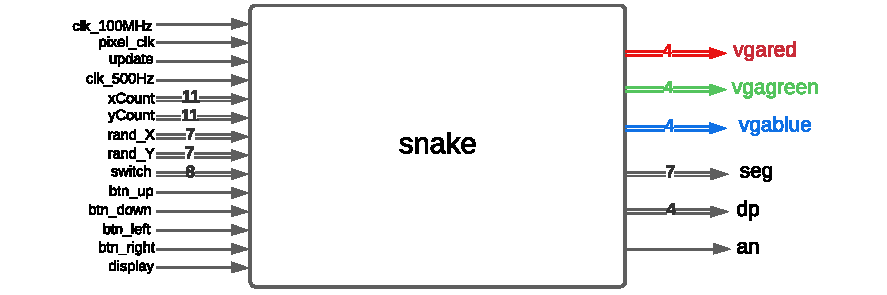
\includegraphics[scale = 0.8]{VGA-Flow - Page 1-1.pdf}
    \caption{\em Inputs/outputs of snake module}
    \label{fig:2}
\end{wrapfigure}

Figure \ref{fig:2} on the left depicts the inputs and outputs of the \verb|snake| module. This module contains the main logic that controls the snake game, as well as the Read Only Memories (ROMs) that store the bitmapped sprites/graphics. The inputs are master 100MHz clock (for synchronisation), pixel clock (25MHz), update clock (25Hz), x and y counters, random food location, and the debounced buttons. It outputs the red, green, blue signals for VGA and the cathode and anode signals for the 7-segment display. 


\begin{figure}[h]
  \centering
  %\captionsetup{justification=centering}
  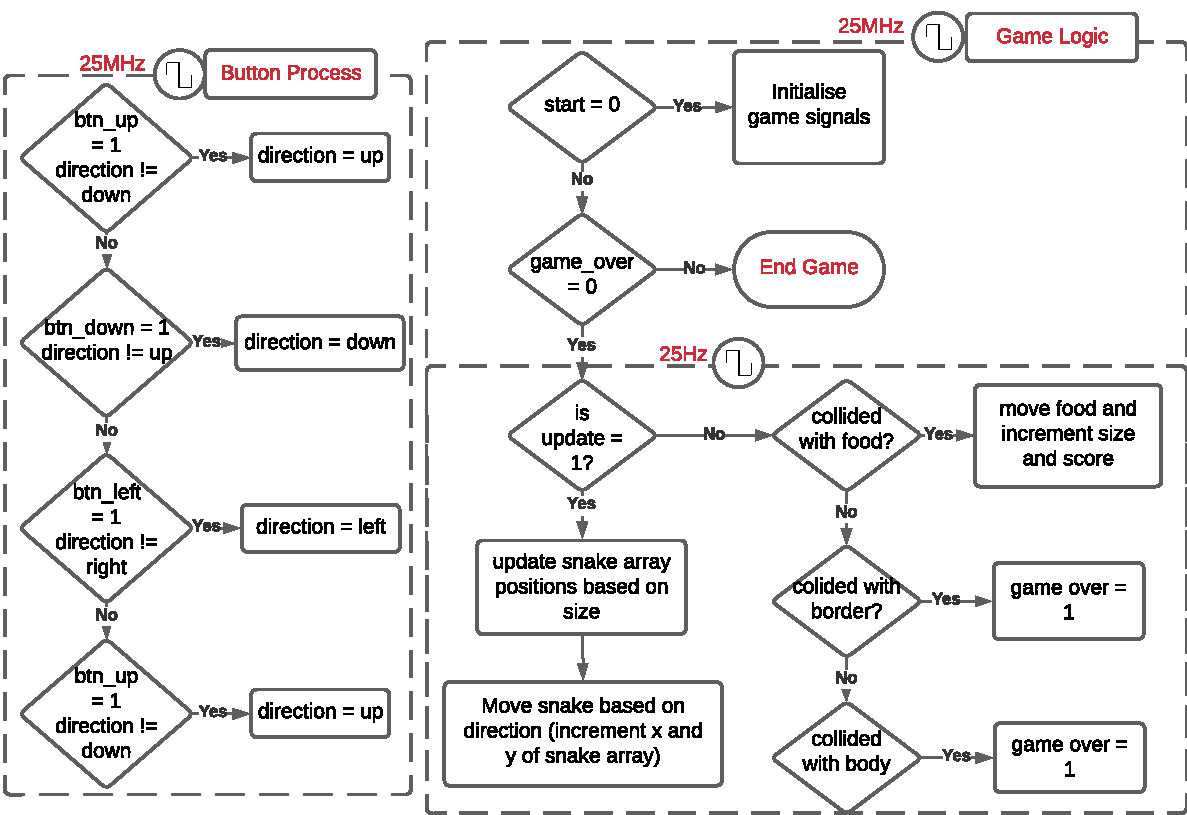
\includegraphics[scale = 0.72]{logic.pdf}
  \caption{\em Button and game logic processes of the snake module}
  \label{fig:3}
\end{figure}

\clearpage

\begin{wrapfigure}[32]{l}{0.5\textwidth}
    \centering
    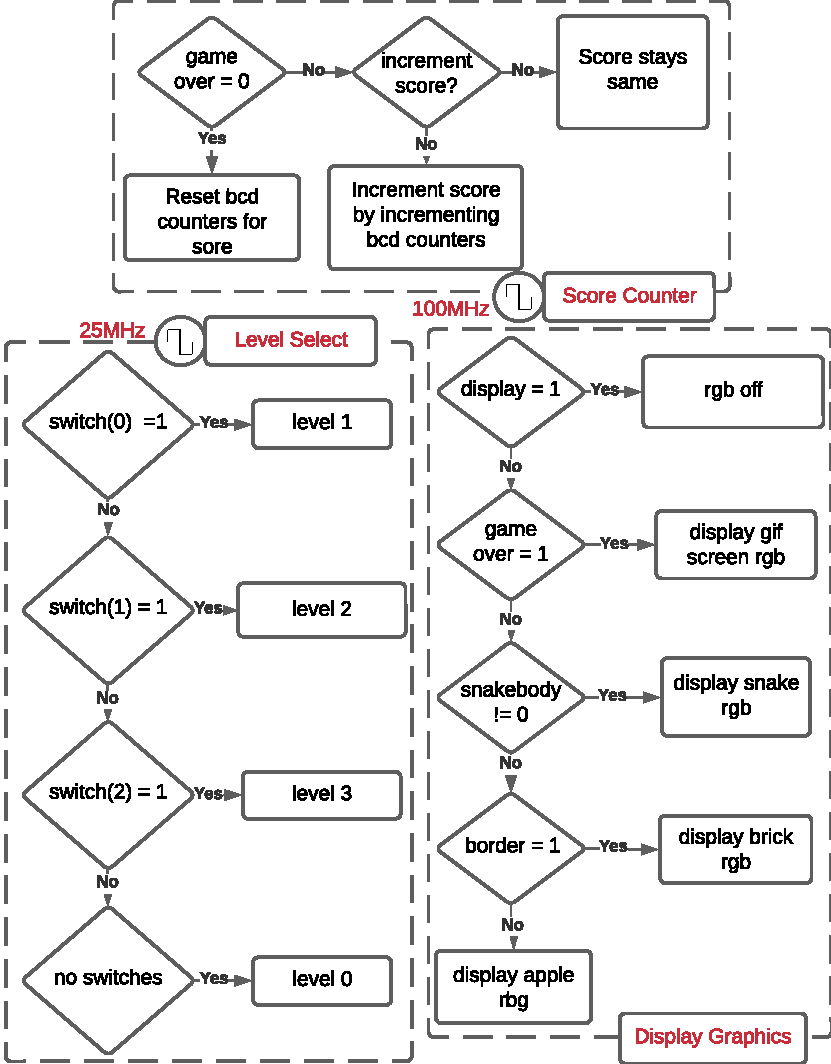
\includegraphics[scale = 0.65]{score.pdf}
    \caption{\em Level select and score count process and colour rendering}
    \label{fig:4}
\end{wrapfigure}

The \verb|snake| module is composed of many processes to construct the game logic and behaviour. Figure \ref{fig:3} and Figure \ref{fig:4} shows flow diagrams to represent this. Figure \ref{fig:3} above shows the button/input and the main game logic process. The button process sets the value of the \verb|direction| register based on the button input. The button input is received from the \verb|Debounce| module (which debounces the button presses for reliability). This process updated with the pixel clock of 25MHz. The game logic process handles updating the snake for the movement as well as checking for collisions. If the start signal is zero, the game is idle and all the starting game conditions are set to defaults (such as initial food location). If the game over signal is high, the game will end until the game is reset, and once reset, the game is reset back to default values. This part of this process is updated at 25MHz. The other parts of the process is updated at 25Hz, which is the games update clock. When the update clock is high, the snake position array (for both x and y locations) are updated in a for loop depending on the current snake size. The snake position at the first index (snake head) is updated depending on the current direction (set by the buttons). When the update clock is low, the collision between the border, food and the snake body is checked. If a collision with the food is detected, the snake size is incremented (unless max snake length is reached). Next if the snake head collides with a border or itself, then the game over signal will be set, thus ending the game, until the game is reset.  Figure \ref{fig:4} shows three other important processes in this module. The score counting process increments the score during the game when food is collected and when the game ends, the game is reset. BCD counters and a 7-segment display driver is used to achieve this. The level select process is very simple, it selects the level based on the switch input. And the levels are border signals that are generated based on certain conditions that decide where the borders are placed on the screen. Lastly, the colour displaying/rendering logic is a combinational process, the other processes we have seen so far are sequential logic. If the display signal is high (same as blanking, which is active low logic), then the RBG colours are turned off. The rgb colours are selected based on which graphics is to be rendered, in this case, the border graphics, the game over GIF and the snake. Graphics in this game are all bitmapped ROMs, this will be explained later in the report. 

\vspace{-1.5em}
\subsubsection{\fontsize{10pt}{12pt}\selectfont \bf updateClk \label{sec:2.2.2}}
\vspace{-1.5em}
% \begin{wrapfigure}[32]{l}{0.5\textwidth}
%     \centering
%     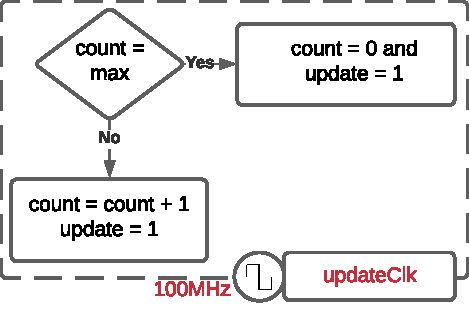
\includegraphics[scale = 0.65]{update.pdf}
%     \caption{\em Level select and score count process and colour rendering}
%     \label{fig:4}
% \end{wrapfigure}

\begin{figure}[h]
\centering
\captionsetup{justification=centering}
\begin{subfigure}{0.5\textwidth}

%   \centering
  %\captionsetup{justification=centering}
  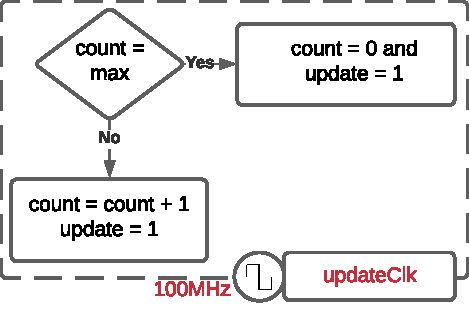
\includegraphics[scale = 0.6]{update.pdf}
  \caption{\em Flow chart for updateClk}

% \caption{\em Diagram of a Differential Drive Mobile Robot}
\label{fig:subim1}
\end{subfigure}
\begin{subfigure}{0.4\textwidth}
%   \centering
  %\captionsetup{justification=centering}
  
\includegraphics[scale = 0.72]{update_block.pdf}
  \caption{\em Entity block of updateClk}
  
% \caption{\em Differential Drive Robot Kinematics}
\label{fig:subim2}
\end{subfigure}
\caption{\em updateClk module diagrams}
\label{fig:5}
\end{figure}

\clearpage

Figure \ref{fig:5} above contains two sub figures, Figure \ref{fig:subim1} and Figure \ref{fig:subim2} which are the architecture and block diagram of this entity respectively. This module has one input, the master clock and one output, the update clock. This is a generic value where the max count can be configured for a different update clock. The update clock used in this game is set to 25Hz. The architecture counts till the set max value and sets the output high for one clock cycle of the master clock, and then becomes low after.

\vspace{-1em}
\subsubsection{\fontsize{10pt}{12pt}\selectfont \bf randomGrid \label{sec:2.2.3}}


\vspace{-1.5em}
\begin{wrapfigure}[7]{l}{0.4\textwidth}
    \centering
    
\includegraphics[scale = 0.85]{random.pdf}
    \caption{\em randomGrid entity diagram}
    \label{fig:6}
\end{wrapfigure}
~\\
Figure \ref{fig:6} on the left shows the inputs and outputs of the randomGrid module. This module is used to generate the pseudo random x and y locations for the food. The pseudo random generation implementation in this project is very simple, as a simple mathematical operation is done on the current random location to move the food `unprediectably'.

\begin{code}
  \label{code:1}
  \captionof*{listing}{Code Snippet 1: {randomGrid architecture implementation}}
  \vspace{-0.5em}
  \begin{minted}
  [
  frame=single,
  framesep=10pt,
  baselinestretch=1.2,
  bgcolor=backgroundColour,
  fontsize={\fontsize{9.5}{6.5}\selectfont},
  % linenos,
  tabsize=2,
  breaklines
  ]
  {vhdl}
if rising_edge(pixel_clk) then
    rand_X <= ((rand_X + 3) mod 37) + 1; -- set random x and y position
    rand_Y <= ((rand_Y + 3) mod 27) + 1;
end if;
  \end{minted}
  \end{code}
  
Since the implementation is simple, it is shown in \hyperref[code:1]{Code Snippet 1}. A simple arithmetic oprtation is computed on the value read back from the current random x and y value, at the rising egde of the pixel clock. The output of this module is given as input to the \verb|snake| module.

\vspace{-1.5em}
\subsubsection{\fontsize{10pt}{12pt}\selectfont \bf 7-Segment Display \label{sec:2.2.4}}

\begin{figure}[h]
  \centering
  %\captionsetup{justification=centering}
  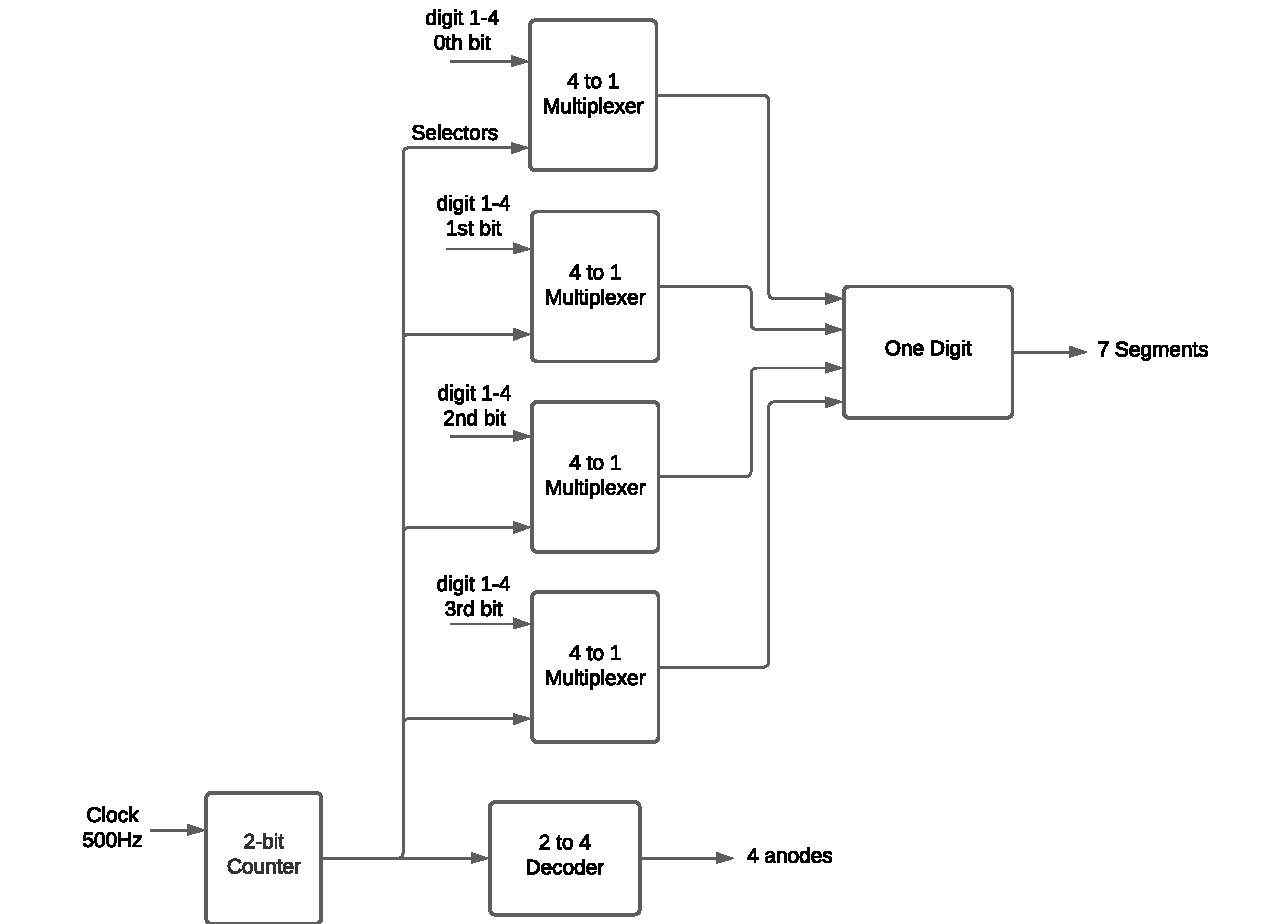
\includegraphics[scale = 0.69]{four_digits.pdf}
  \caption{\em Architectural block diagram of the four\_digits module}
  \label{fig:7}
\end{figure}

\clearpage

\begin{wrapfigure}[9]{l}{0.42\textwidth}
  \centering
  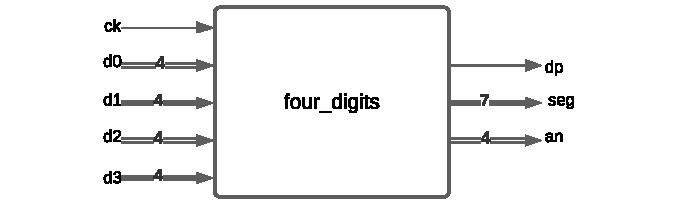
\includegraphics[scale = 0.8]{four_digit_block.pdf}
  \caption{\em four\_digits entity diagram}
  \label{fig:8}
\end{wrapfigure}

This section explains the 7-segment display driver (and it's subcomponents) circuit used to display the score. Figure \ref{fig:8} on the left shows the entity inputs and outputs and Figure \ref{fig:7} above shows the high level connection diagram. This module takes in a 500Hz clock, and four inputs which are four bits wide, and generates the required anode and cathode displays. Time division multiplexing is used to display the four digits on the four seven segment displays available on the Basys3 board. The 500Hz clock given to a two bit counter which counts from 0$\rightarrow$3, and it's output is fed into a 4-t0-1 multiplexer to select the corresponding bit for that digit. The four multiplexer output is given to a module called \verb|one_digit| which is a 7-segment decoder. The 2-bit counter output is also used by a 2-to-4 decoder to select the correct anode which is currently being displayed. The anodes are swapped at a rate of 500Hz, a refresh rate human eyes cannot visibly see. The 2-bit counter being very simple is implemented using behavioural modelling. Figure \ref{fig:9}, \ref{fig:10} and \ref{fig:11} below shows the entity block diagrams of \verb|mux4_1|, \verb|decoder2_4| and \verb|one_digit| respectively, which is used in the circuit from Figure \ref{fig:7}.

\begin{figure}[!htb]
  \minipage{0.32\textwidth}
    
\includegraphics[width=\linewidth]{mux4.pdf}
    \caption{\em mux4\_1 entity}\label{fig:9}
  \endminipage\hfill
  \minipage{0.32\textwidth}
    
\includegraphics[width=\linewidth]{dec.pdf}
    \caption{\em decoder\_2\_4 entity}\label{fig:10}
  \endminipage\hfill
  \minipage{0.32\textwidth}%
    
\includegraphics[width=\linewidth]{one_digit.pdf}
    \caption{one\_digit entity}\label{fig:11}
  \endminipage
  \end{figure}
  
All the three modules are very simple. \verb|one_digit| takes in a 4 bit number as input and outputs the corresponding 7 bit output for the 7 segments on the 7-segment display. The \verb|decoder| entity is a simple two-to-four decoder, a certain bit of the 4 bit output is low depending on the input. For example, if the input is $01_2$, the output is $1101_2$, the $2^{\text{nd}}$ bit is low. And lastly, the 4-to-1 mux routes the corresponding bit of the input \verb|a| depending on the select input \verb|s|, to the output. The \verb|four_digit| module is instantiated inside the \verb|snake| module from Figure \ref{fig:2} and its outputs are propagated outside the \verb|snake| module.

\vspace{-1em}
\subsubsection{\fontsize{10pt}{12pt}\selectfont \bf Debounce \label{sec:2.2.5}}

\begin{figure}[h]
\centering
\captionsetup{justification=centering}
\begin{subfigure}{0.5\textwidth}

%   \centering
  %\captionsetup{justification=centering}
  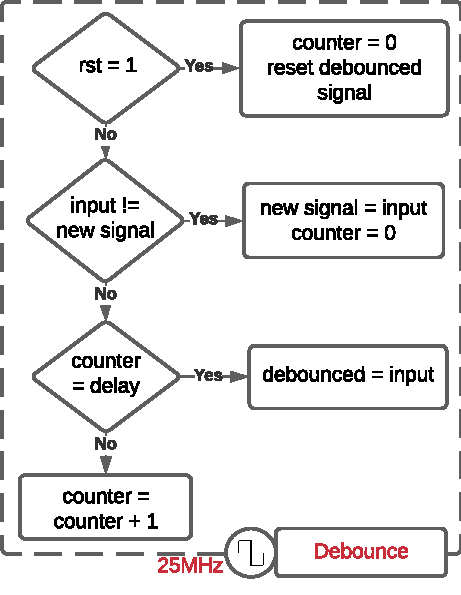
\includegraphics[scale = 0.6]{debounce_flow.pdf}
  \caption{\em Flow chart for Debounce}

% \caption{\em Diagram of a Differential Drive Mobile Robot}
\label{fig:subim3}
\end{subfigure}
\begin{subfigure}{0.4\textwidth}
%   \centering
  %\captionsetup{justification=centering}
  
\includegraphics[scale = 0.72]{debounce.pdf}
  \caption{\em Entity block of Debounce}
  
% \caption{\em Differential Drive Robot Kinematics}
\label{fig:subim4}
\end{subfigure}
\caption{\em Debounce module diagrams}
\label{fig:12}
\end{figure}

Figure \ref{fig:subim3} and \ref{fig:subim4} shows the flow chart and entity diagram for the Debounce module respectively. There are three inputs, clk, rst and noisy (the button input) and one output which is thd debounced press. This module has a configurable generic parameter, \verb|DELAY|. This module is clocked at the pixel clock, 25MHz. The module has a counter that counts till a delay value is reached, and once the count is same as the delay, the button press is debounced, and the counter is reset. The debounced output is input to the \verb|snake| module.

\clearpage

\subsubsection{\fontsize{10pt}{12pt}\selectfont \bf vga\_controller\_640\_60 \label{sec:2.2.6}}


\vspace{-1.5em}
\begin{wrapfigure}[10]{l}{0.45\textwidth}
    \centering
    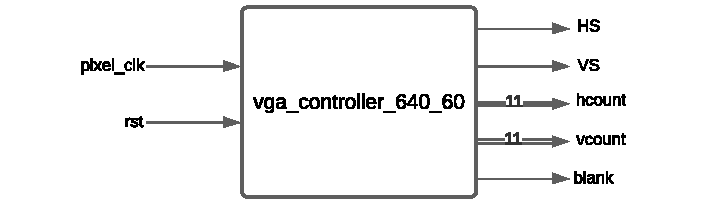
\includegraphics[scale = 0.8]{vga_controller.pdf}
    \caption{\em VGA Controller module}
    \label{fig:13}
\end{wrapfigure}
~\\
Figure \ref{fig:13} on the left shows the entity diagram of the \verb|vga_controller_60_40| module. This module wasn't written by the author and was given by the supervisor. This module has 2 inputs, the 25MHz pixel clock (\verb|pixel_clock|) and reset (\verb|rst|). And outputs the horizontal sync (\verb|HS|), vertical sync \verb|VS|, current horizontal counter value (\verb|hcount|), current vertical counter value (\verb|vcount|) and the blanking signal (\verb|blank|). The horizontal and vertical synchronisation signals are outputted to the VGA port in the top level hierarchy. The vertical counter, horizontal counter and the blanking signals are all given as inputs to the \verb|snake| module from \ref{fig:2} to control the game logic.

\vspace{-1em}
\subsubsection{\fontsize{10pt}{12pt}\selectfont \bf nbit\_clk\_div \label{sec:2.2.7}}
\vspace{-0.5em}
\begin{figure}[h]
\centering
\captionsetup{justification=centering}
\begin{subfigure}{0.5\textwidth}

%   \centering
  %\captionsetup{justification=centering}
  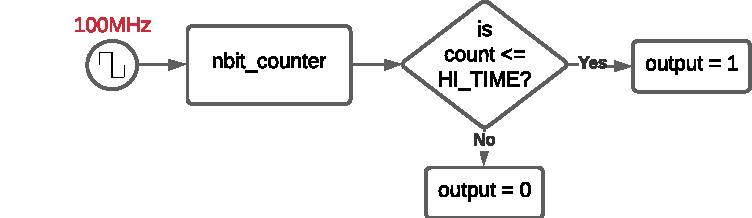
\includegraphics[scale = 0.6]{clk-block.pdf}
  \caption{\em Flow chart for nbit\_clk\_div}

% \caption{\em Diagram of a Differential Drive Mobile Robot}
\label{fig:subim5}
\end{subfigure}
\begin{subfigure}{0.4\textwidth}
%   \centering
  %\captionsetup{justification=centering}
  
\includegraphics[scale = 0.72]{clk_div.pdf}
  \caption{\em Entity block of nbit\_clk\_div}
  
% \caption{\em Differential Drive Robot Kinematics}
\label{fig:subim6}
\end{subfigure}
\caption{\em nbit\_clk\_div module diagrams}
\label{fig:14}
\end{figure}

Figure \ref{fig:14} above shows the flow diagram and entity diagram of the \verb|nbit_clk_div| module (Figure \ref{fig:subim5} and \ref{fig:subim6} respectively). There is one input, the clock and one output, the divided clock. This module is a configurable and generic which is configurable, such as the division factor and the duty cycle. This is possible because the module instantiates another module called \verb|nbit_counter| inside it, which also a generic component. The counter is clocked at 100Mhz (the master clock) and the output is compared with the configured highest count. If the counter reaches a value within a certain threshold, it makes the output high, else makes it low. And the constant \verb|HI_TIME| is calculated from a generic value \verb|high_count|, to control the duty cycle as per the user's usage.

\begin{wrapfigure}[7]{l}{0.35\textwidth}
    \centering
    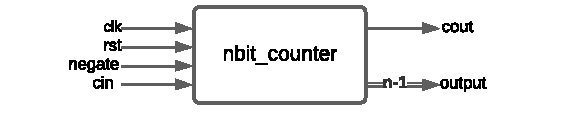
\includegraphics[scale = 0.8]{counter.pdf}
    \caption{\em nbit\_counter module}
    \label{fig:15}
\end{wrapfigure}
~\\
Figure \ref{fig:15} on the left-hand side shows the generic counter used inside the clock divider. It has a configurable maximum count value. It is a very general purpose module as it has a \verb|negate| input, and the \verb|cin| input and \verb|cout| output can be used to easily chain multiple counters. The output of this module is used in the clock divider module in order to generate the divided clock signal. 

\vspace{-1em}
\subsubsection{\fontsize{10pt}{12pt}\selectfont \bf nbit\_bcd\_counter \label{sec:2.2.8}}

\vspace{-1em}
\begin{wrapfigure}[7]{l}{0.37\textwidth}
  \centering
  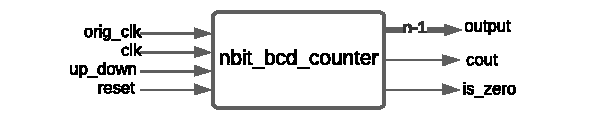
\includegraphics[scale = 0.8]{bcd.pdf}
  \caption{\em nbit\_bcd\_counter module}
  \label{fig:16}
\end{wrapfigure}
~\\
Figure \ref{fig:16} on the left shows the entity block diagram of the \verb|nbit_bcd_counter| module, which is a generic BCD counter which is configurable from a maximum count between 0$\rightarrow$99. This module is used to keep track of the score as the snake eats the food objects. The implementation of this module is very simple, inside it are two modulo-10 counters that are cascaded. When one modulo-10 counter reaches it's $1001_2$ (in up count) or $0000_2$ (in down count), the second counter is incremented or decremented respectively. There are 3 inputs, the original master clock (\verb|orig_clk|, to help with synchronisation), the clock (\verb|clk|) at which the counter is incremented, \verb|up_down| to swap between up and down count mode, and \verb|reset|. The \verb|is_zero| output is not used. This module is instantiated inside the \verb|snake| module, and two are instantiated (as there are 4 7-segment displays) and are cascaded using the \verb|cout| output. The output of the 2 BCD counters are inputs to the \verb|four_digits| module.

\clearpage

\subsubsection{\fontsize{10pt}{12pt}\selectfont \bf Bitmapped Sprites and GIFs \label{sec:2.2.9}}

As mentioned in section \ref{sec:2.2.1} of this report, graphics used in this game are stored as bitmap ROMs. This section details how sprites as well as GIFs were rendered on the VGA monitor. Bitmaps were used to render sprites and GIFs on the screen. A bitmap is essentially an array that holds information for each pixel in the image. In the case of this design, each element in the array holds RGB colour value for each pixel. 

\begin{code}
  \label{code:2}
  \captionof*{listing}{Code Snippet 2: {\em ROM used for the snake sprite}}
  \vspace{-0.5em}
  \begin{minted}
  [
  frame=single,
  framesep=10pt,
  baselinestretch=1.2,
  bgcolor=backgroundColour,
  fontsize={\fontsize{7.5}{6.5}\selectfont},
  % linenos,
  tabsize=2,
  breaklines
  ]
  {vhdl}
type color_sprite_8 is array (0 to 7, 0 to 7) of std_logic_vector(0 to 11);
constant SNAKE_ROM : color_sprite_8 := (
	("010101100010","011010000010","011010000010","011010000010","011010000010","011010000010","011010000010","001001010001"),
	("011010000010","010011000001","001110110001","001110110001","001110110001","001110110001","001110110001","001001100001"),
	("011010000010","001110110001","000110100001","000110100000","000110100000","000110100001","000110100000","001001100001"),
	("011010000010","001110110001","000101110001","001010100001","001010100001","001001110001","001010100001","001001100001"),
	("011010000010","001110110001","000110100001","001010010001","001010010001","001010100001","001010110000","001001100001"),
	("011010000010","001110110001","000110100001","001010100001","001010100001","001010100001","001010110000","001001100001"),
	("011010000010","001110110001","000110110000","001010110000","001010110000","001010110000","001010110000","001001100001"),
	("001001010001","001001100001","001001100001","001001100001","001001100001","001001100001","001001100001","000101010001")
);
  \end{minted}
  \end{code}

\hyperref[code:2]{Code Snippet 2} above shows the ROM implemented to display the snake sprite. A sprite ROM is essentially a two dimensional array where the width and height represents the size of the sprite. In this case it is eight by eight. And each element is an RGB colour value. The ROM is indexed using the x and y counter values, and then is rendered at the desired location. Rendering static sprites is very simple, but it gets slightly tricky when trying to render animated sprites. An animated sprite contains multiple images, hence the bitmap array is an array of two-dimensional arrays.

\begin{code}
  \label{code:3}
  \captionof*{listing}{Code Snippet 3: {\em Type definition for a GIF with 2 frames}}
  \vspace{-0.5em}
  \begin{minted}
  [
  frame=single,
  framesep=10pt,
  baselinestretch=1.2,
  bgcolor=backgroundColour,
  fontsize={\fontsize{8.5}{6.5}\selectfont},
  % linenos,
  tabsize=2,
  breaklines
  ]
  {vhdl}
type apple_gif_sprite is array (0 to 1, 0 to 15, 0 to 15) of std_logic_vector(0 to 11);
  \end{minted}
  \end{code}

Due to page space constraints, only the type definition is shown in \hyperref[code:3]{Code Snippet 3} above. The above syntax defines a 16 by 16 sprite with 2 frames. And in this case, both the frame and the individual pixel colour in the bitmap needs to be indexed. A simple counter signal is used to index the current frame of the animated sprite. Within the current frame, the x and y counter values are used to get the RGB colour value.\\
These bit maps are generated by a Python script which takes in a GIF or PNG and generates VHDL ROM syntax. Which is then included in the code. All the ROMS are stored in the file \verb|snake.vhd| which is shown in \hyperref[code:snake]{Source Code 2} in the \hyperref[sec:app]{Appendix}.. And the python scripts are in \hyperref[code:py]{Source Code 15} and \hyperref[code:py2]{Source Code 16} in the \hyperref[sec:app]{Appendix} as well.

\vspace{-0.7em}
\subsection{\fontsize{11.4pt}{12pt}\selectfont \bf Development Process \label{sec:2.3}}

This section describes the steps taken to develop the hardware design as well as what issues were faced and how they were rectified. First, the given VGA driver source code and simple colour rendering was tested, by attempting to display a solid red colour. This can be seen in the GitLab commit linked \href{https://cseegit.essex.ac.uk/23-24-ce339/23-24_CE339_gopinath_akshay/-/commit/41b12159ecd4fd75b2ae10749d8d0f7c15da76b0}{here}. \\
\\
After this, the main snake game logic was developed. As seen from this \href{https://cseegit.essex.ac.uk/23-24-ce339/23-24_CE339_gopinath_akshay/-/commit/911c4fae4d40bebe5094a92a998859baa51b185a}{GitLab commit} link, the colour rendering was not working initially, and some attempts were made to try and rectify this problem. The first attempt was to try making the sequential logic more reliable by following the discussion shown in reference [7]. Apparently in VHDL, it is better to synchronise most logic to the master clock of the board (thus rising edge of the 100MHz clock), and use the output of the clock divider as an enabler signal. This is because the synthesiser interprets the output of a clock divider as a normal `wire' and not as a `clock'. Although this didn't fix the issue after \href{https://cseegit.essex.ac.uk/23-24-ce339/23-24_CE339_gopinath_akshay/-/commit/18064c441e06b2e87fbe97886cf5f8ecc04e3233}{this commit}, this is a good VHDL coding practice regardless. This issue was later rectified in \href{https://cseegit.essex.ac.uk/23-24-ce339/23-24_CE339_gopinath_akshay/-/commit/08e170dc860f38bff83c3967aa89f9bca4223632}{this commit}. Where in the render logic for the border, an \verb|or| logic was used instead of \verb|and| logic. Which was a silly mistake. Another fix was made in the same commit, where the movement logic was fixed because the x and y movement of the snake was inverted. \\
~\\
The next  bug discovered was that the game would randomly end (game over) whilst the snake was in motion. This was initally beleived to be a synchronisation problem, but the input process was already clocked to the master clock (with the pixel clock as an enabler). To fix this issue, a button debouncing module was created in \href{https://cseegit.essex.ac.uk/23-24-ce339/23-24_CE339_gopinath_akshay/-/commit/2c20b371731b9e364c1e1e8525bab0f203cde461}{this commit}. But not all the buttons were connected to this module. This bug was fixed in \href{https://cseegit.essex.ac.uk/23-24-ce339/23-24_CE339_gopinath_akshay/-/commit/9eff36c14714be44cf6d5e24563ecbe0abaf9896}{this commit} when all four movement buttons were debounced using the module. This highlights the importance of debouncing button presses. \\

Next, rendering sprites and more complex graphics was attempted. First monochrome sprite rendering was attempted, and as seen from \href{https://cseegit.essex.ac.uk/23-24-ce339/23-24_CE339_gopinath_akshay/-/commit/a958a1af9c4bc434596a061d44baa802a9002064}{this commit}, it wasn't working properly on the first try. The sprite appeared to be enlarged and had to be resized. This was later rectified in a \href{https://cseegit.essex.ac.uk/23-24-ce339/23-24_CE339_gopinath_akshay/-/commit/f787fa3ce0e1d44e9f0805a759b5dafe5140fda9}{later commit}, when the rendering logic was given a context of the size of the image rather than using bit splicing. After this was fixed, coloured sprite rendering was added, as seen from \href{https://cseegit.essex.ac.uk/23-24-ce339/23-24_CE339_gopinath_akshay/-/commit/4a8f2602f10cfca06351e9e81d6a3dccfbe525a5}{this commit}. The RGB rendering logic had to be modified, so that there is one signal for colour that can be spliced to separate signals. After a sprite was added for the borders, one more fixed had to be added for the first level of the game, as shown in \href{https://cseegit.essex.ac.uk/23-24-ce339/23-24_CE339_gopinath_akshay/-/commit/72ade113022557aec48fa33dec5331c03ee3bdc1}{this commit}. Where the first level border generation border signal had to have a context of the sprite size. Lastly, the apple and game over screen GIFs were added. Since the logic for this was exactly the same, this worked as expected on the first attempt. ~\\

To understand how to render complex on an FPGA, the website from reference [6] was used. This website teaches the design approach in SystemVerilog rather than VHDL, but all the concepts depicted in the website carried over nicely, and the logic and theory was easily translatable to VHDL. ~\\

The sprite texture used for the food is shown in reference [2], for the brick/border in reference [3] and for the snake body in reference [4].

\vspace{-0.5em}
\subsection{\fontsize{11.4pt}{12pt}\selectfont \bf Possible Design Improvements \label{sec:2.4}}

There are many places where the current hardware design can be improved. For example the current pseudo random location generation uses a very simple arithmetic operation to `randomise' the location of the food. A smarter approach would have been to use a Linear Feedback Shift Register (LFSR) design as shown in reference [7], which is a very popular approach in both hardware and software to generate random numbers. The current apprach was chosen due to simplicity, and works well. And also due to time contraints for the project. ~\\
~\\
The next improvement that could be made with more time is the visuals of the game. The snake sprite could have been animated and also add a textured background to the game, rather than a solid black background. This was not done again due to time constraints but this shouldn't be hard to adapt into the current code base, as rendering sprites and even animated GIFs has been achieved in this project. ~\\
~\\
The snake source code shown in \hyperref[code:snake]{Source Code 2} could also be improved. As all the ROMs are stored in this one file, it makes the file rather large in terms of lines of code. The ROMs could have possibly been stored elsewhere, maybe a separate entity. This would improve code reliability.

\clearpage


\section{\fontsize{11.3pt}{12pt}\selectfont \bf Testing and Final Results}
\fontsize{11pt}{12pt}\selectfont \label{sec:3}

\begin{figure}[h]
  \centering
  %\captionsetup{justification=centering}
  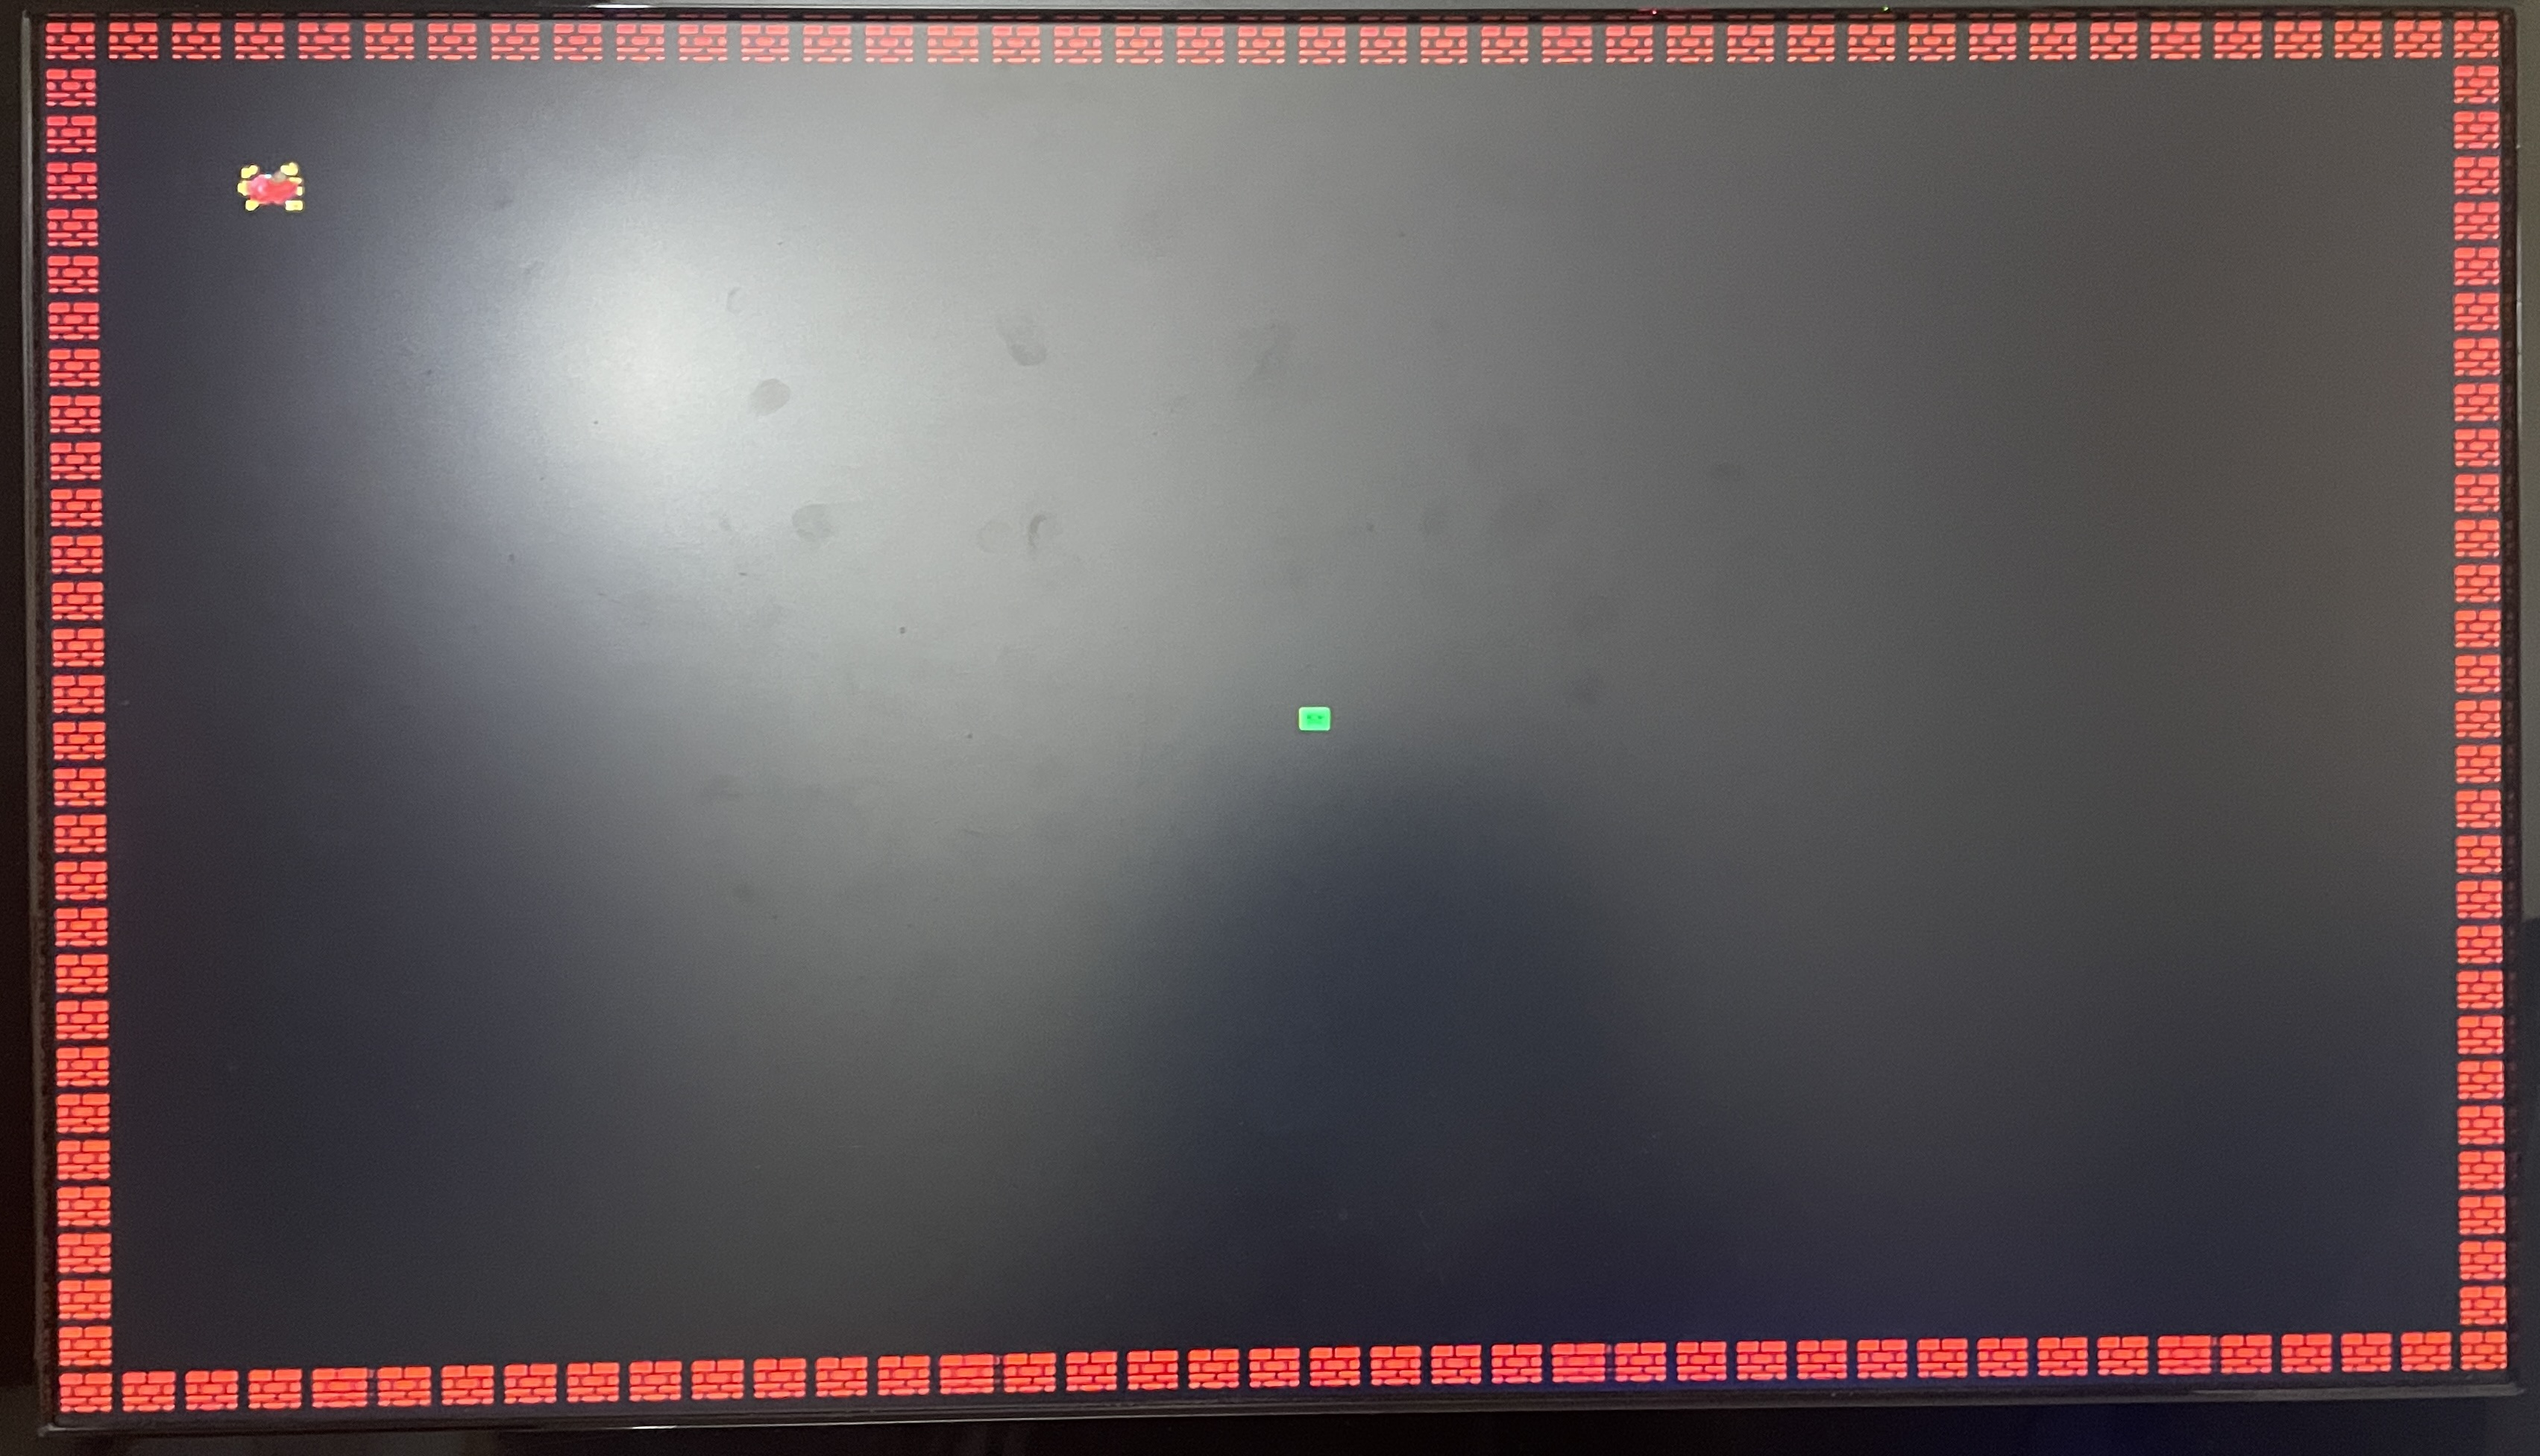
\includegraphics[scale = 0.5]{stationary.jpg}
  \caption{\em When game is stationary}
  \label{fig:17}
\end{figure}

\begin{figure}[h]
  \centering
  %\captionsetup{justification=centering}
  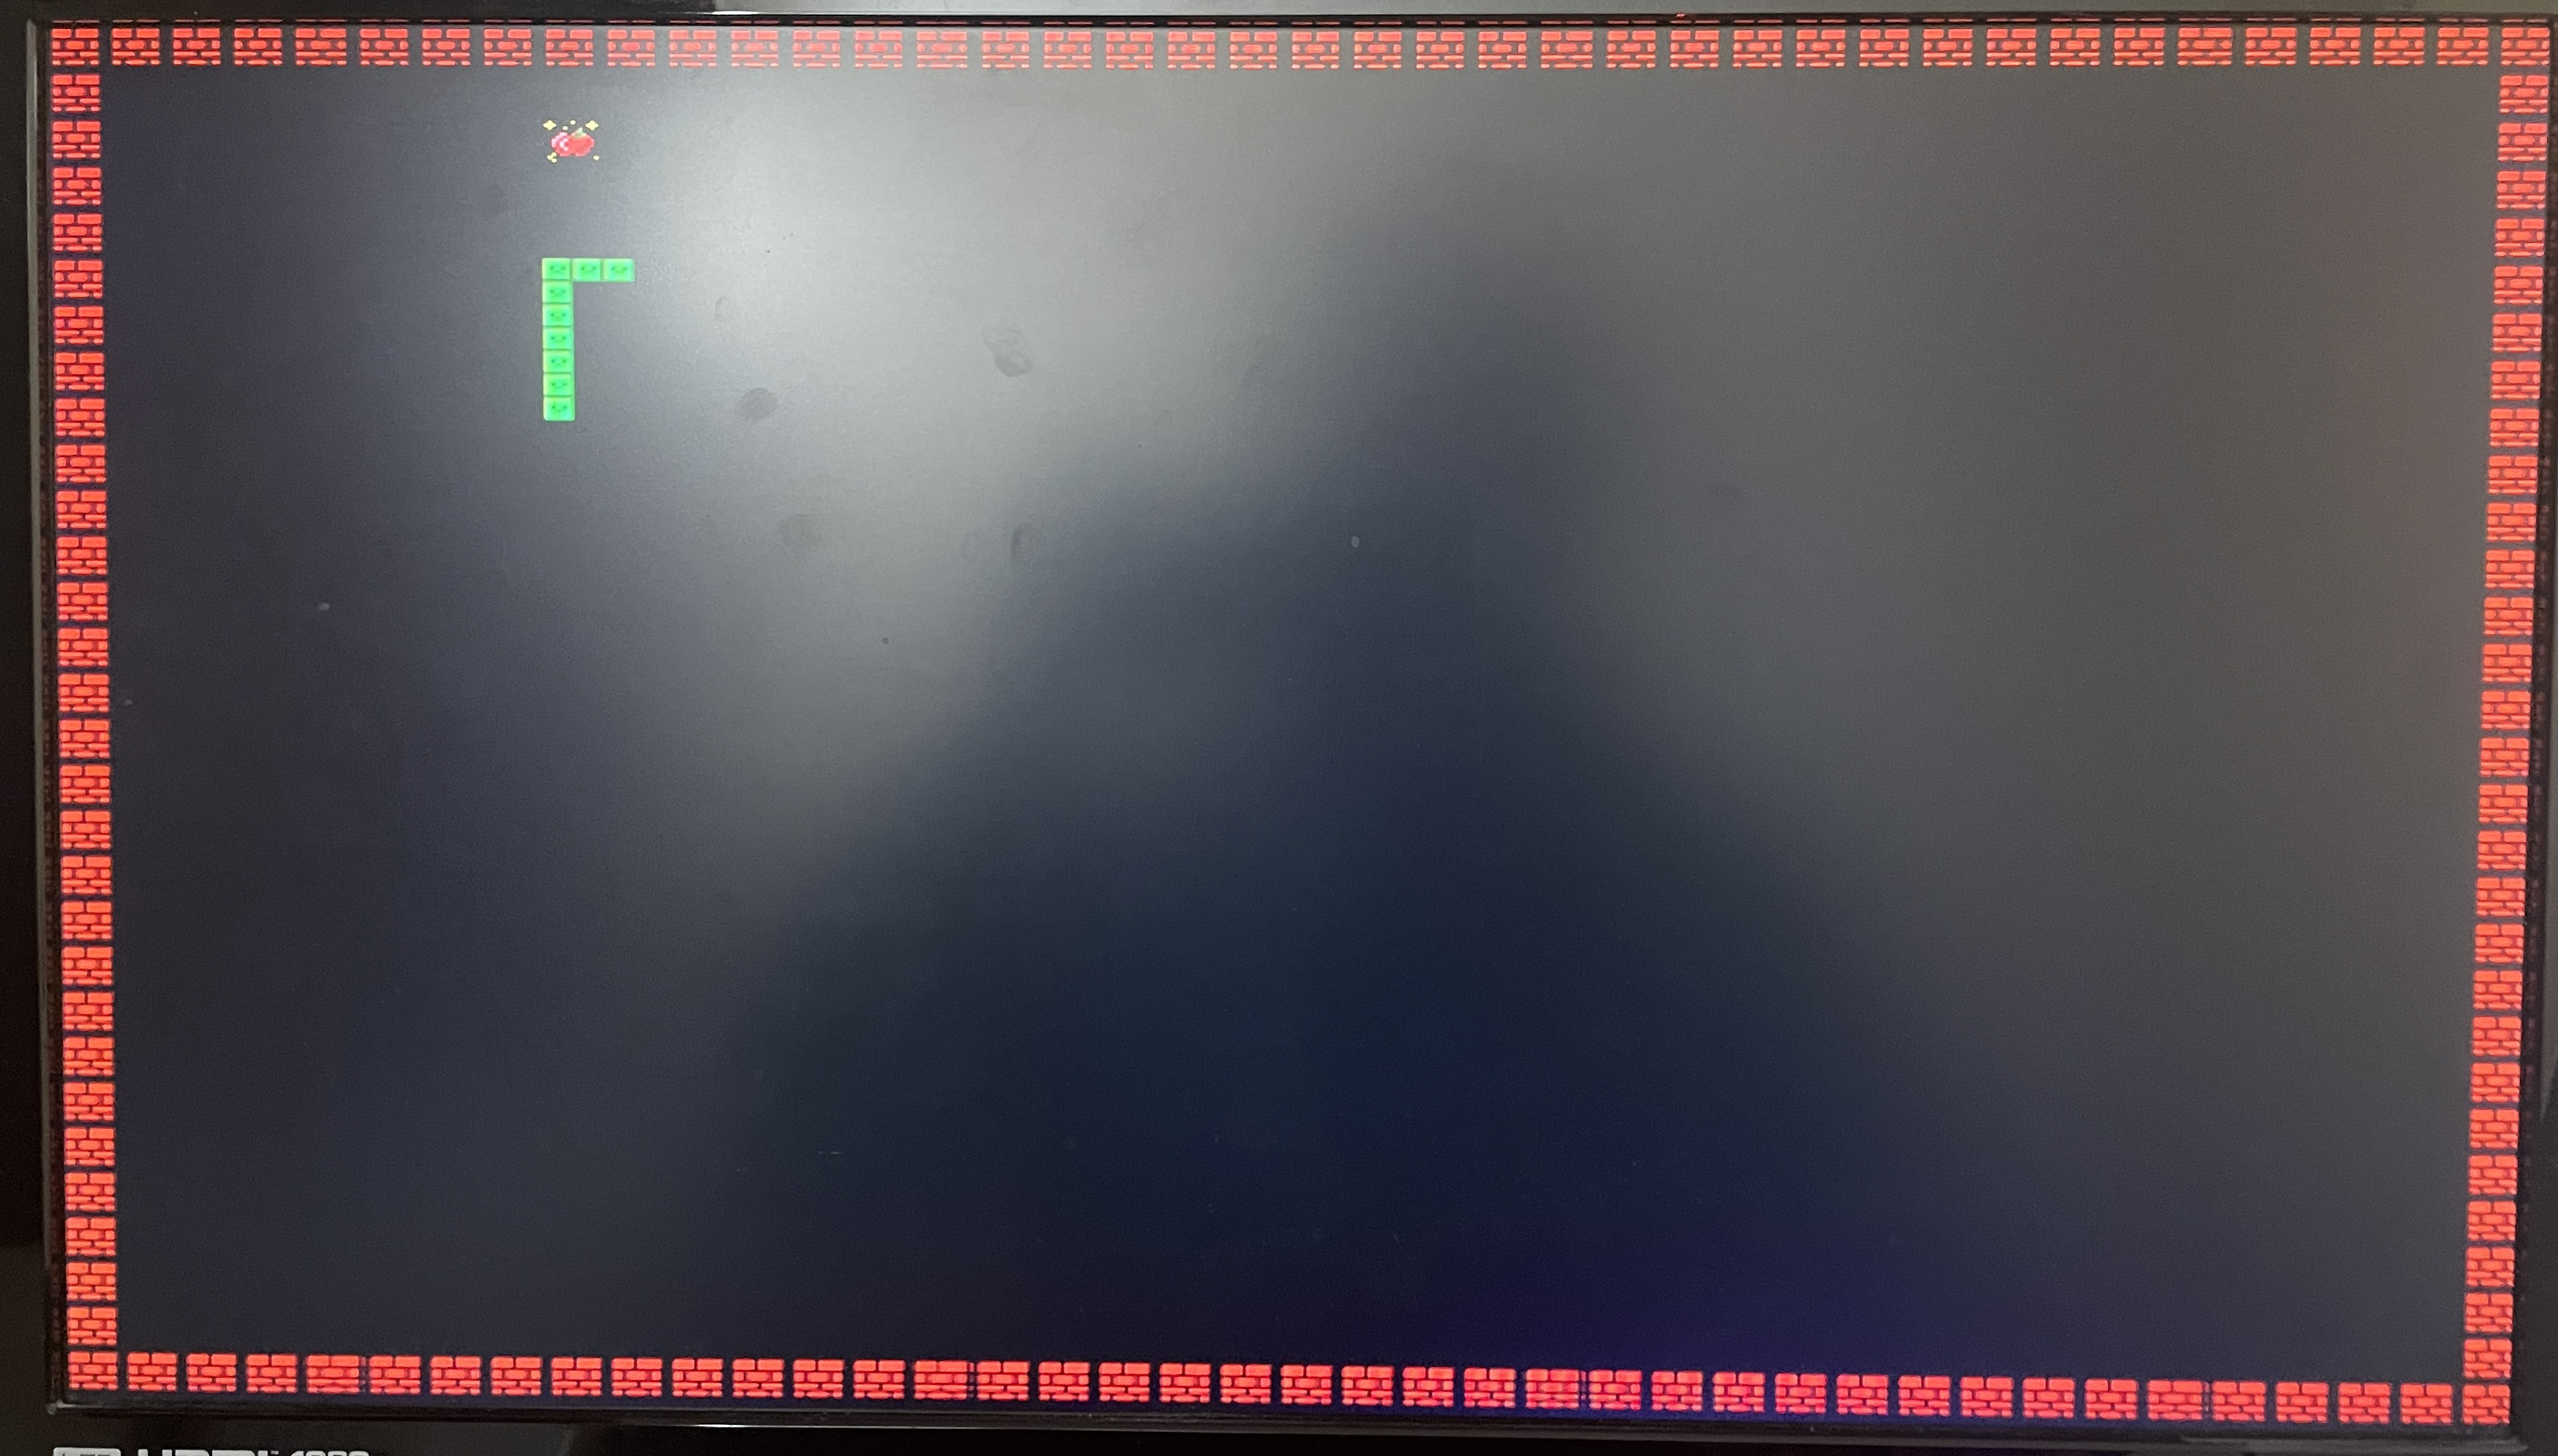
\includegraphics[scale = 0.5]{moving.jpg}
  \caption{\em When game is moving}
  \label{fig:18}
\end{figure}

\clearpage

\begin{figure}[h]
  \centering
  %\captionsetup{justification=centering}
  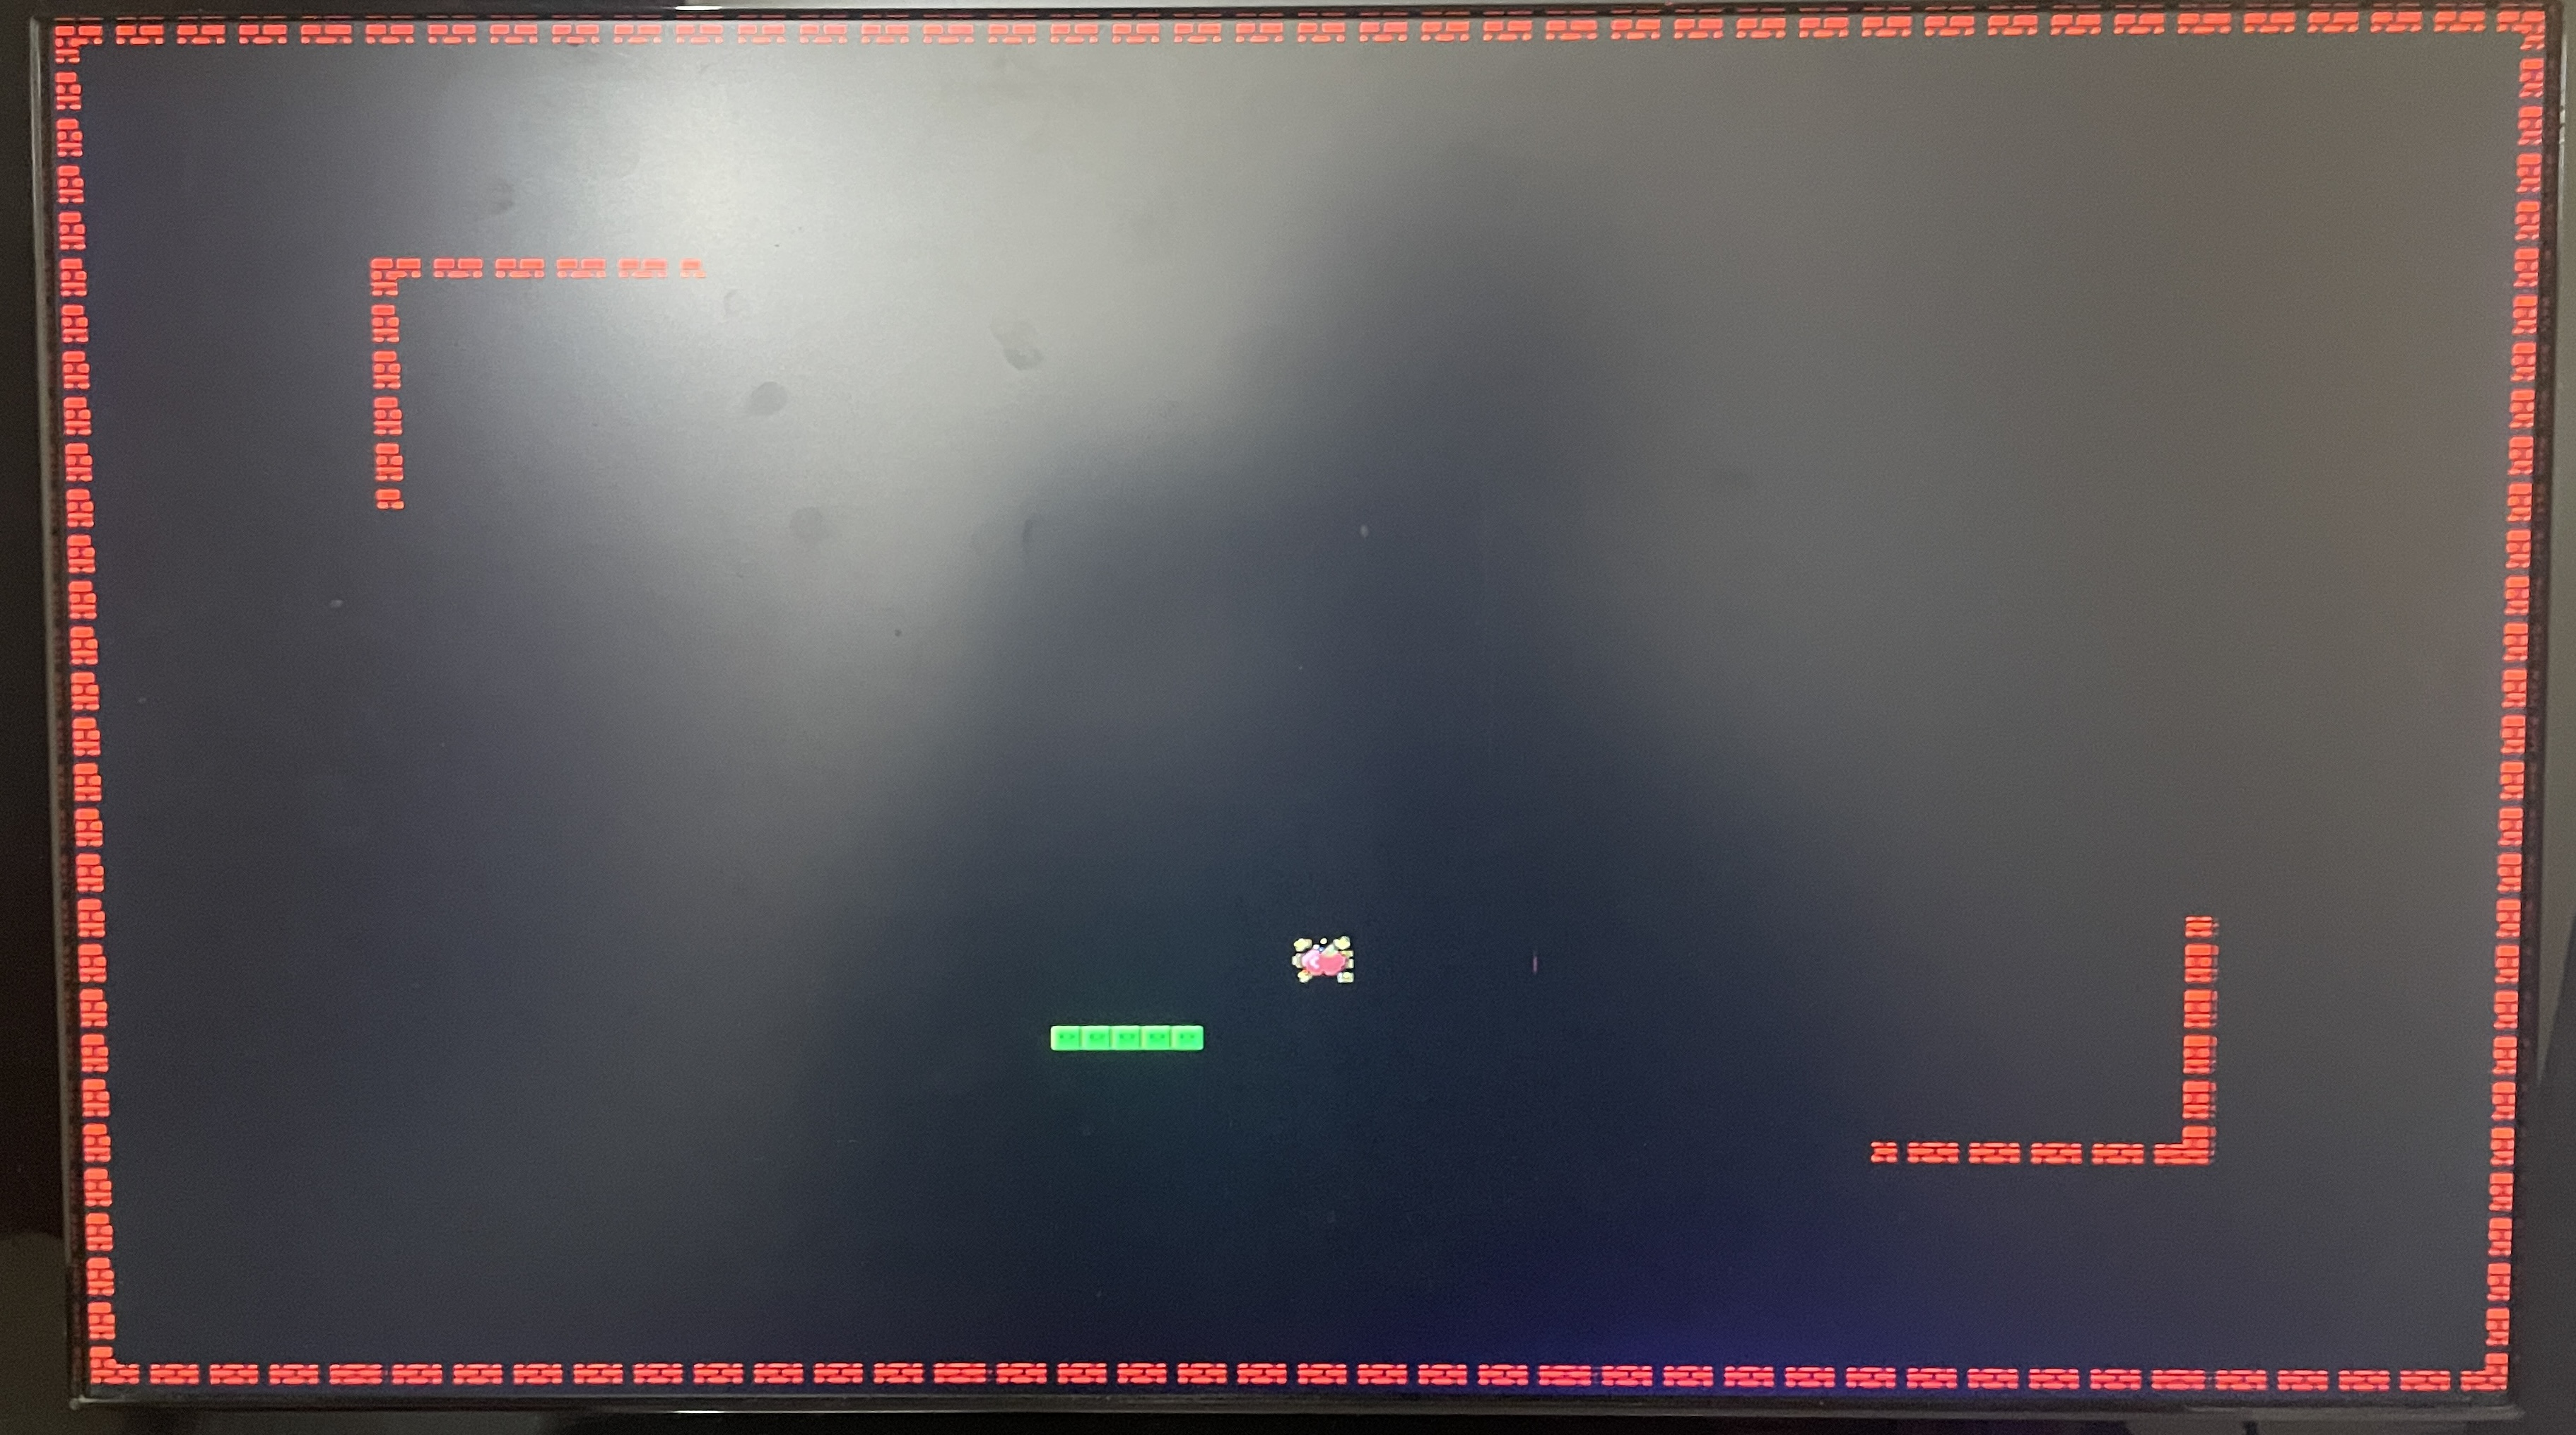
\includegraphics[scale = 0.5]{level.jpg}
  \caption{\em One of the game levels}
  \label{fig:19}
\end{figure}

\begin{figure}[h]
  \centering
  %\captionsetup{justification=centering}
  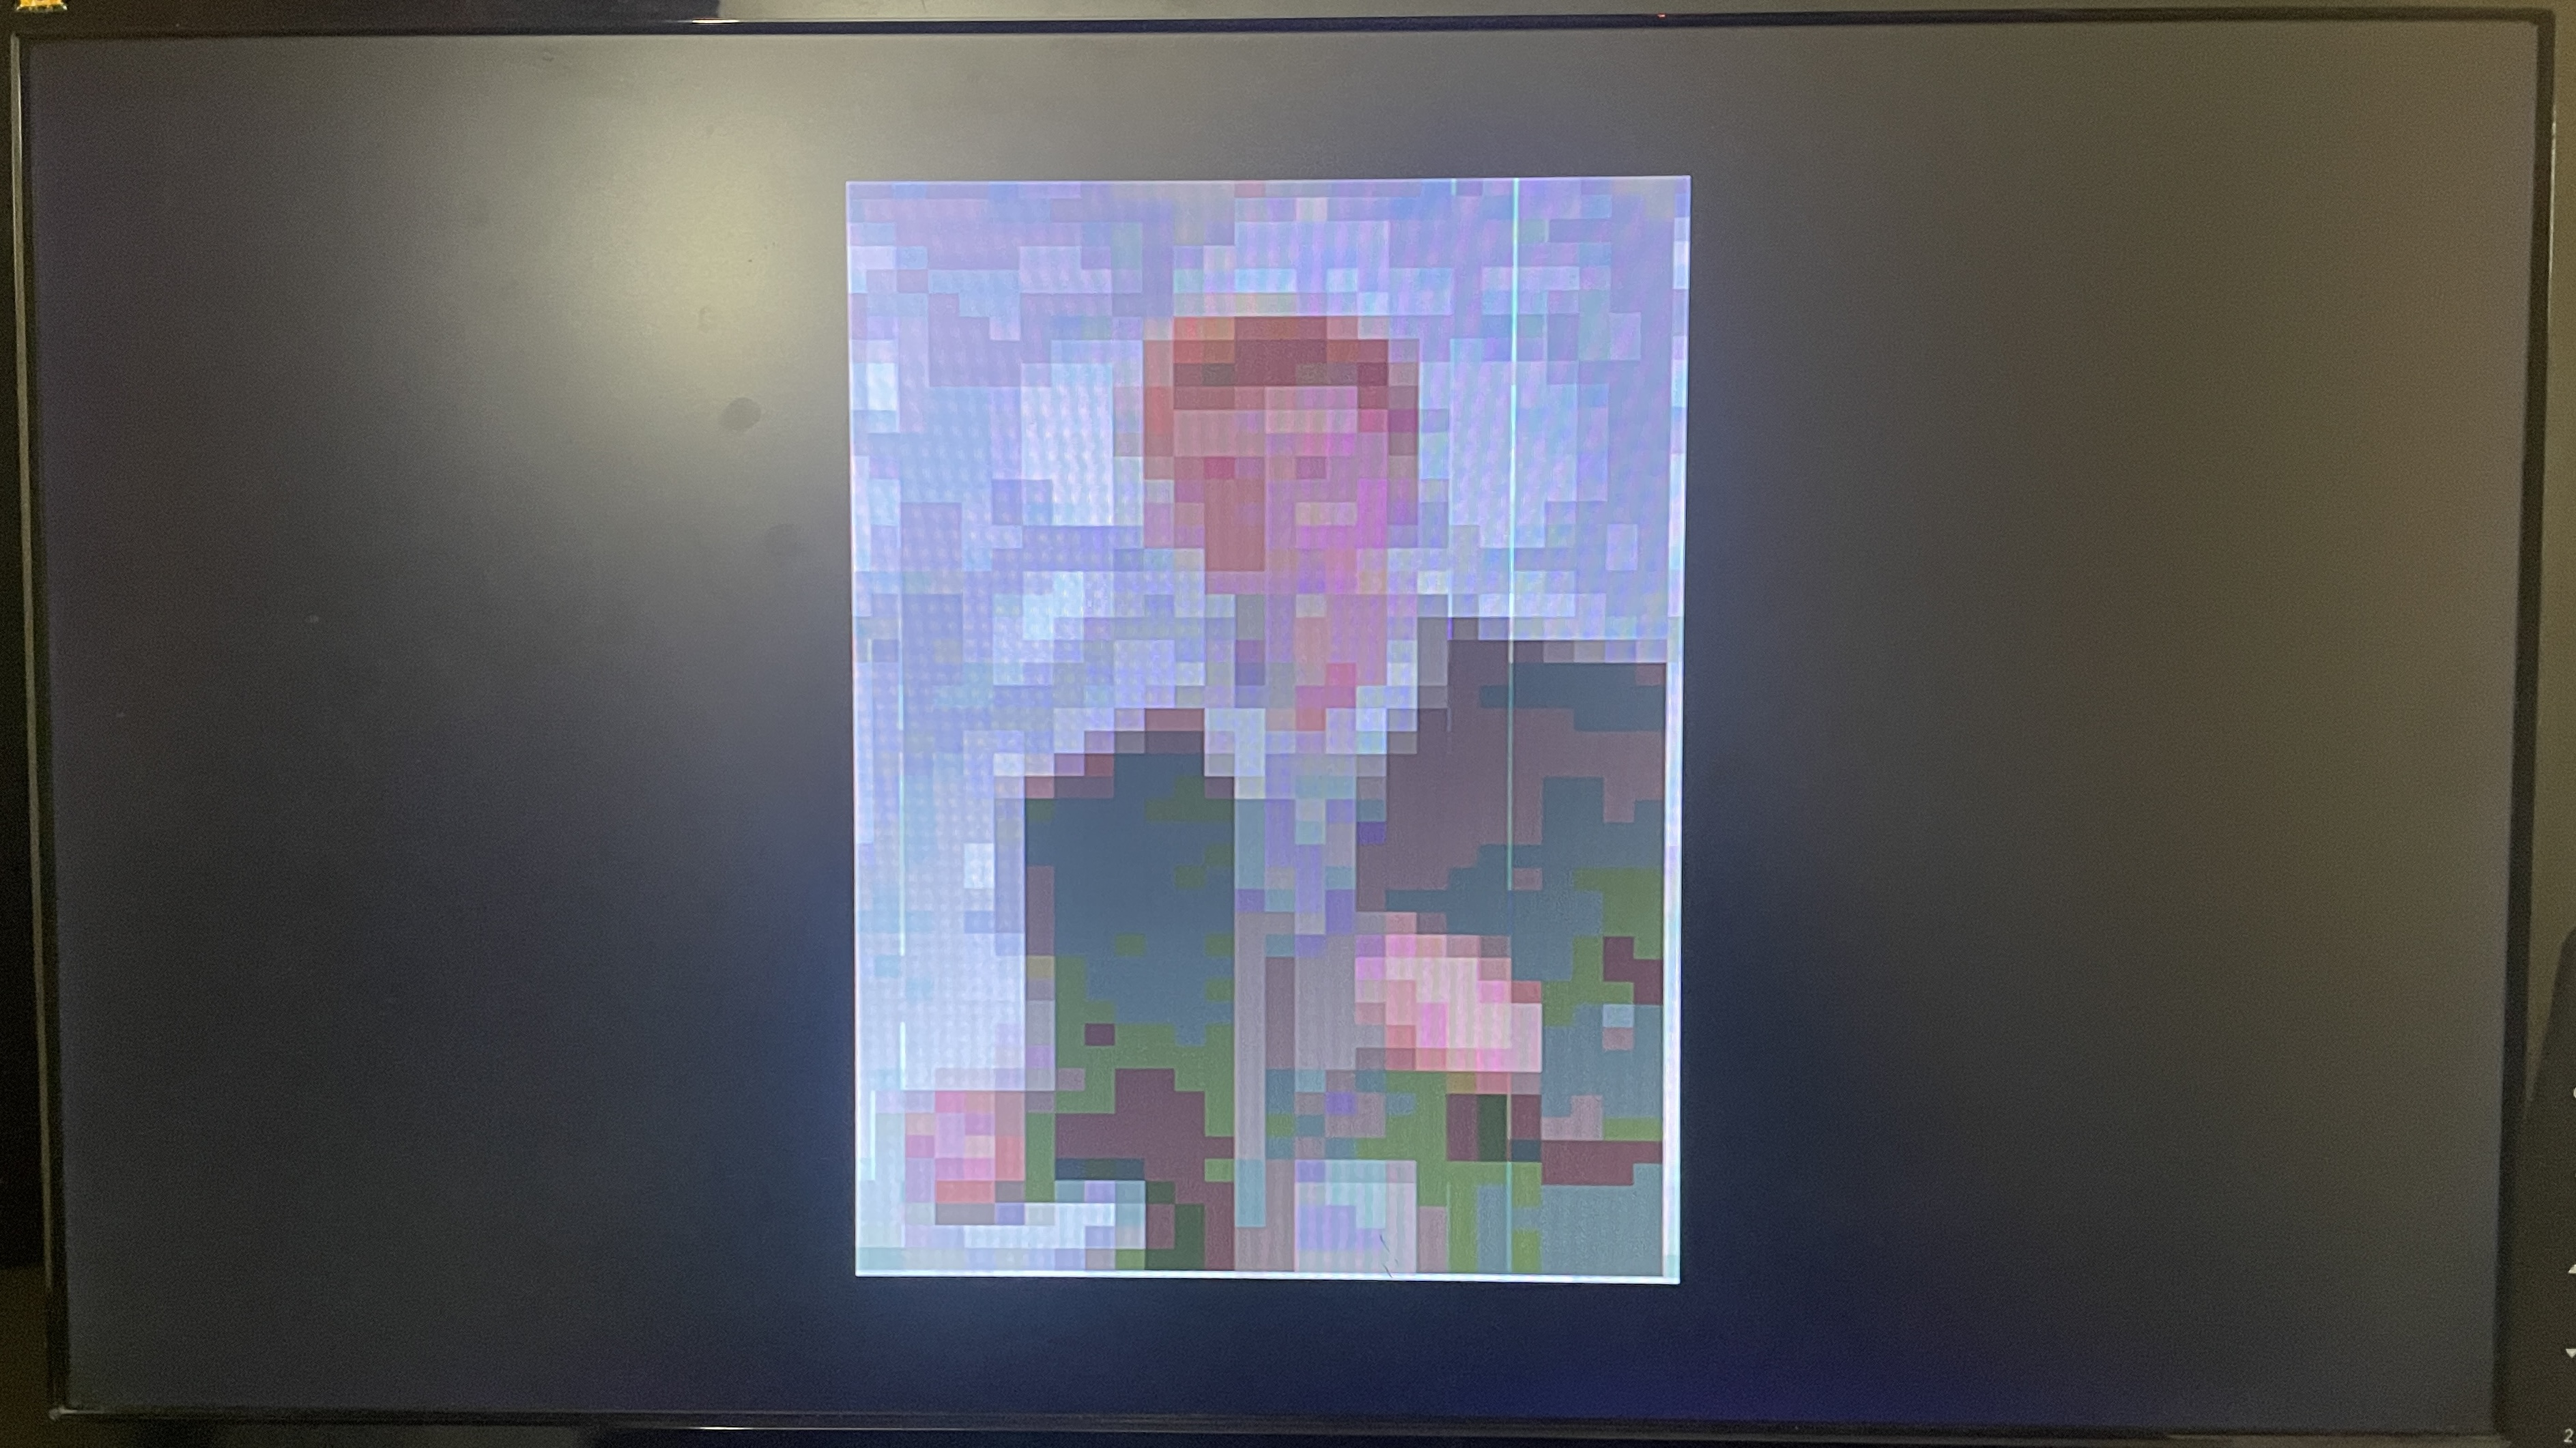
\includegraphics[scale = 0.5]{over.jpg}
  \caption{\em Game over screen}
  \label{fig:20}
\end{figure}

\clearpage

\begin{figure}[h]
  \centering
  %\captionsetup{justification=centering}
  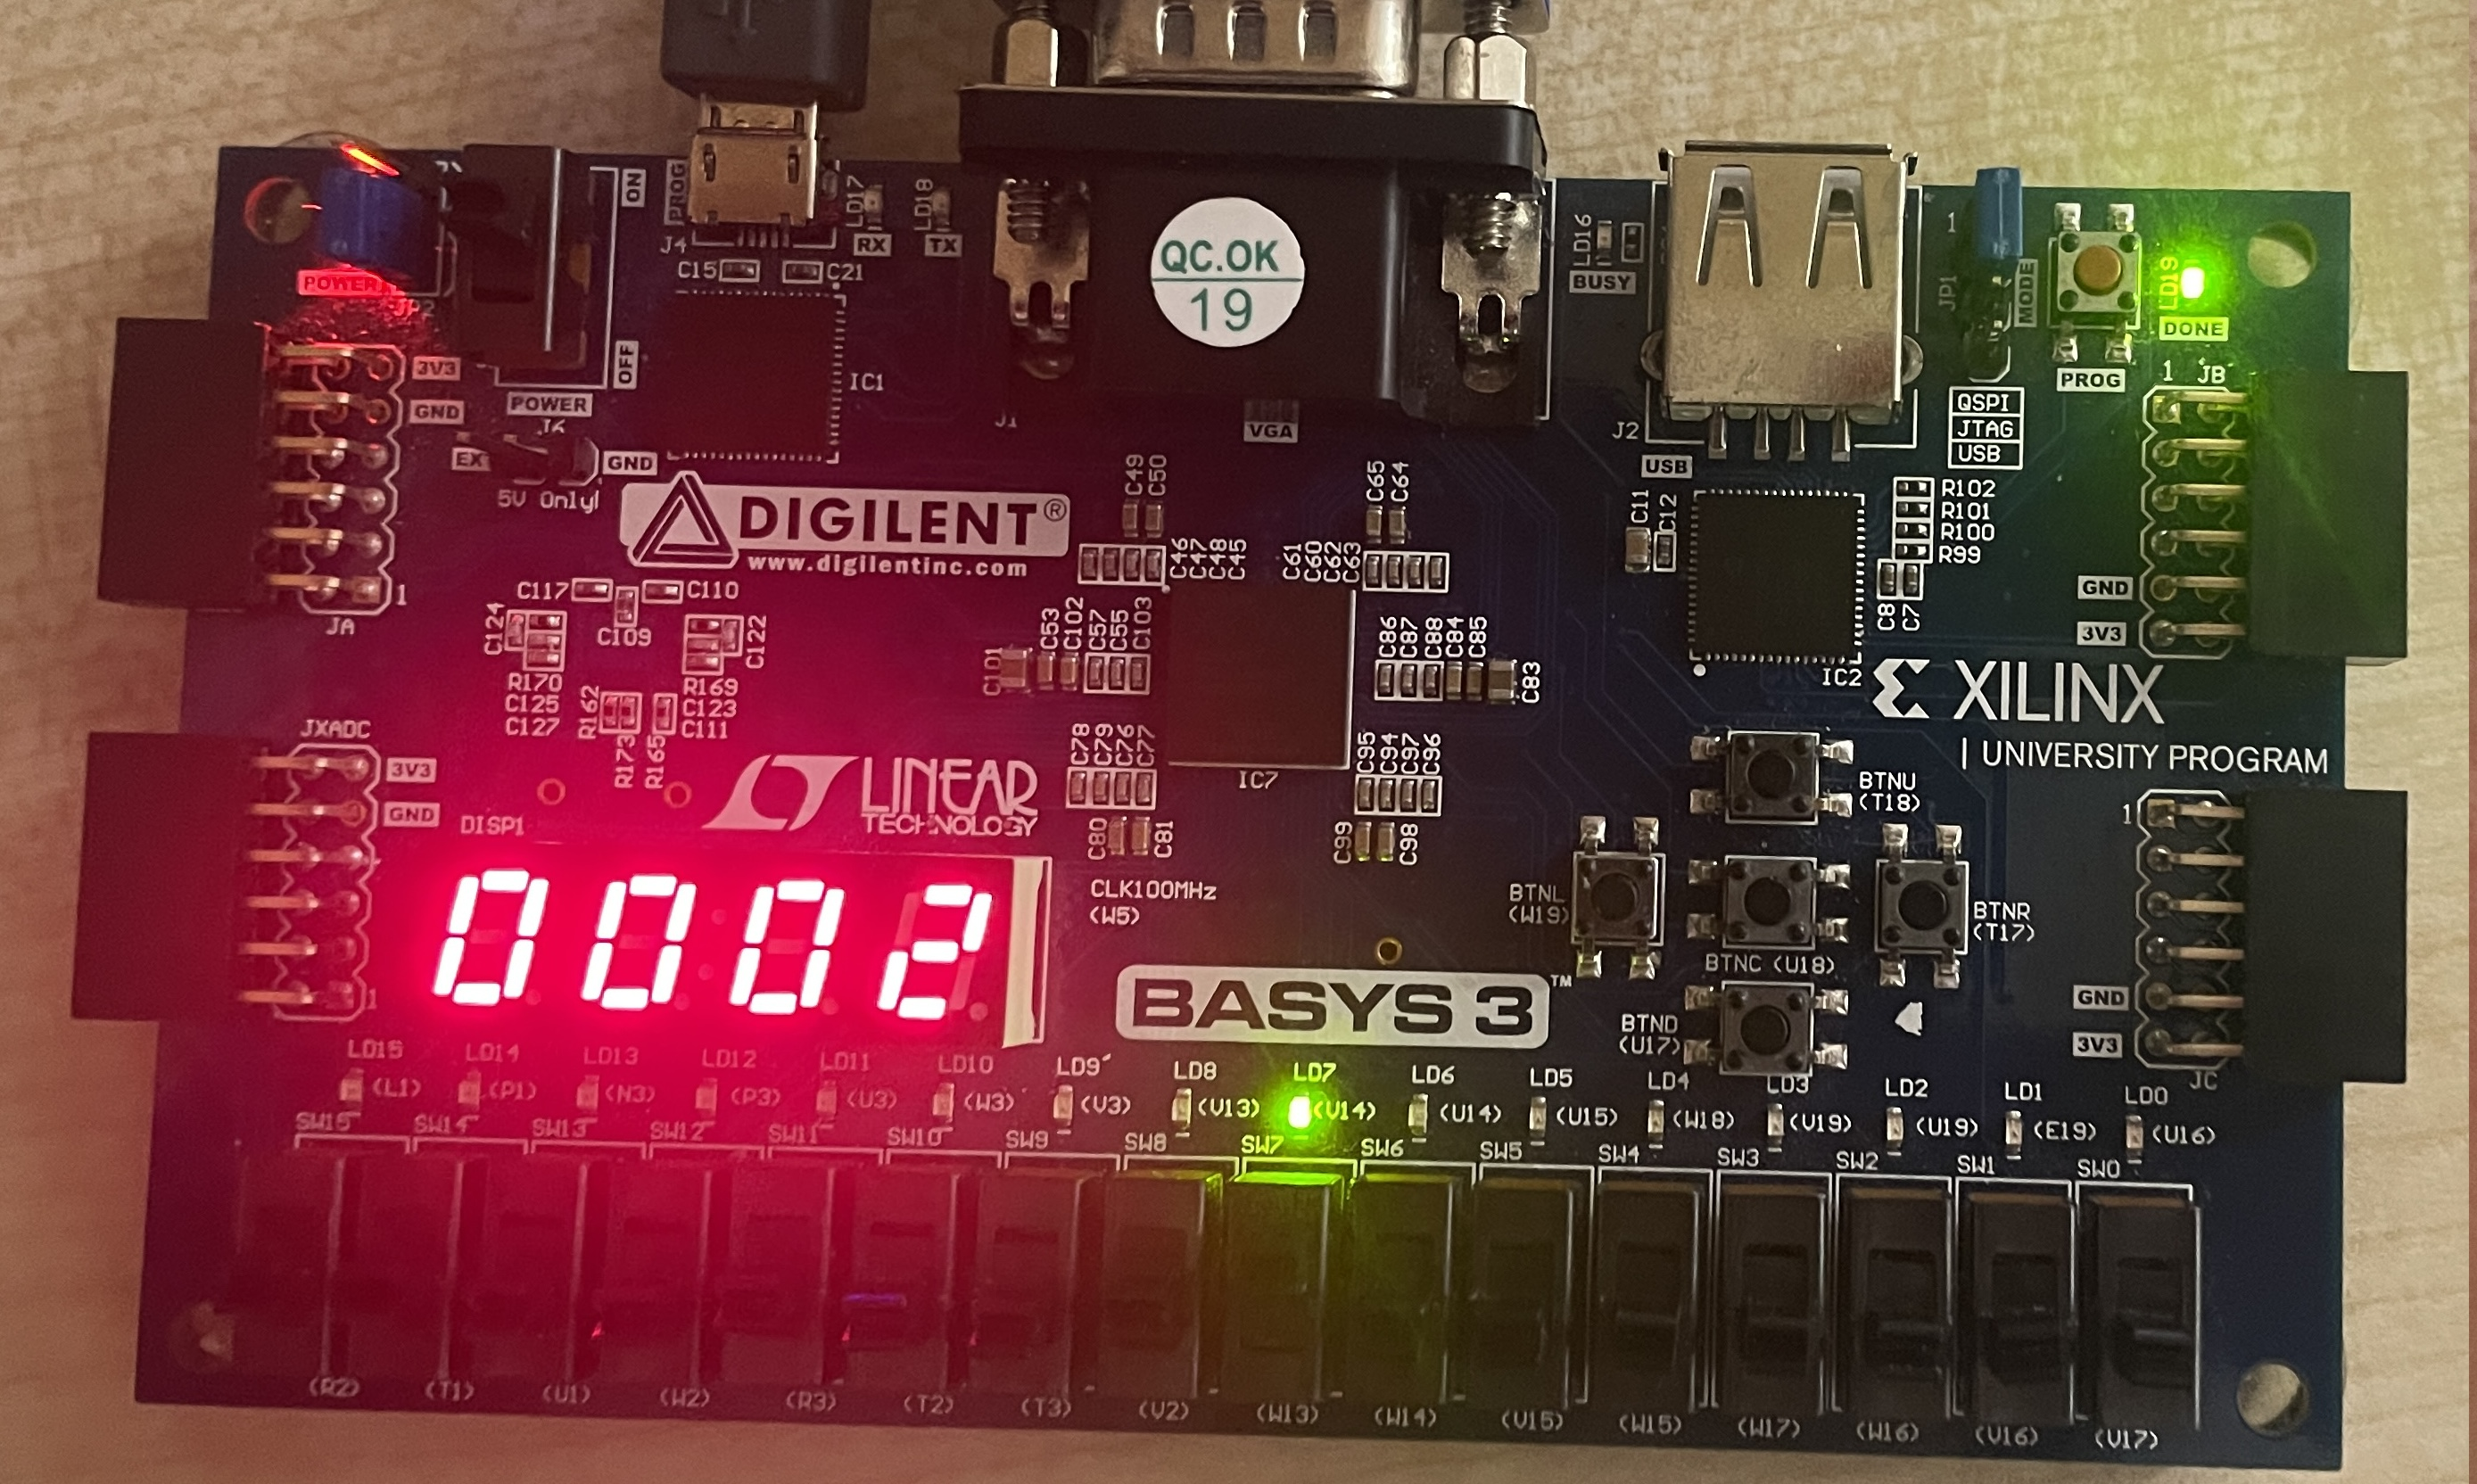
\includegraphics[scale = 0.6]{score.jpg}
  \caption{\em Displaying the score on the 7-segment display}
  \label{fig:20}
\end{figure}

{\large \bf A video/gif showcase can be seen in the GitLab repo README page linked \href{https://cseegit.essex.ac.uk/23-24-ce339/23-24_CE339_gopinath_akshay/-/tree/master/assignment_2}{here}}


\clearpage

\section{\fontsize{11.3pt}{12pt}\selectfont \bf Conclusion}
\fontsize{11pt}{12pt}\selectfont \label{sec:4}


By the end of the project, a playable and functional snake game was implemented with hardware static and animated sprites as well as multiple levels. Both the VGA graphics (to display the game) and the 7-segment display (to show the player score) worked successfully and as expected. This can be seen from the pictures from Section \ref{sec:3} of the report.~\\

There is a lot to learn from this project. First is observing how the VGA standards work, such as the synchronisation signals, its timings and how the RGB colours raster is used to produce graphics. With the use of memory systems, in this case ROMs (Read Only Memory), bitmaps can be stored so that they can be indexed to display both static and animated sprite based graphics. The usage and the workings of 7-segment displays and how time division multiplexing can be used to control multiple displays with one set of pins, was also observed. ~\\


Another important lesson learnt is how hierarchical and modular based design can be used to design a digital system. In this case, every distinct logic has been attempted to be split into separate entities to allow for a modular design with an easy-to-follow hierarchy from top to low level. For example, using separate entities for circuits such as button debouncing, clock divider, snake game logic etc.~\\


Often in engineering, first iterations are not always bug free or even functional. And a design will need to go through different patches in order to reach a functional/playable state. And this was the case for this project as well, as showcased in \ref{sec:2.3} of this report. And this highlights the importance of using a version control system, in this case Git in order to keep track of changes within the source code that is being developed.~\\

Overall, this project was successfully implemented with great results, just like every other engineering project, has scope for future extensions and improvements.


\clearpage


\section{\fontsize{11.3pt}{12pt}\selectfont \bf References}
\fontsize{11pt}{12pt}\selectfont \label{sec:5}

[1] S. K, ``Basys 3,'' Basys 3 - Digilent Reference, \url{https://digilent.com/reference/programmable-logic/basys-3/start} (accessed Mar. 26, 2024). 

[2] RndmWeirdo, “A shiny apple? by rndmweirdo on DeviantArt,” by RndmWeirdo on DeviantArt, \url{https://www.deviantart.com/rndmweirdo/art/A-shiny-Apple-840730109} (accessed Mar. 26, 2024). 

[3] BloodyYoshi, “Super Mario Bros HD - brick block by bloodyyoshi on DeviantArt,” by BloodyYoshi on DeviantArt, \url{https://www.deviantart.com/bloodyyoshi/art/Super-Mario-Bros-HD-Brick-Block-740859067} (accessed Mar. 26, 2024). 

[4] Super Mario Wiki, “Snake block,” Super Mario Wiki, \url{https://www.mariowiki.com/Snake\_Block} (accessed Mar. 26, 2024). 

[5] “Linear-feedback shift register,” Wikipedia, \url{https://en.wikipedia.org/wiki/Linear-feedback\_shift\_register} (accessed Mar. 26, 2024). 

[6] W. Green, “FPGA \& RISC-V Tutorials,” Project F, \url{https://projectf.io/tutorials/} (accessed Mar. 26, 2024).

[7] user1175889user1175889                      14133 gold badges44 silver badges1313 bronze badges, Martin ThompsonMartin Thompson                      16.6k11 gold badge3838 silver badges5757 bronze badges, and sonicwavesonicwave                      6, “Making a clock divider,” Stack Overflow, \url{https://stackoverflow.com/questions/19708301/making-a-clock-divider} (accessed Mar. 26, 2024). 

\clearpage


\section{\fontsize{11.3pt}{12pt}\selectfont \bf Appendix}
\fontsize{11pt}{12pt}\selectfont \label{sec:app}

{\large {\bf Note: For the file \hyperref[code:snake]{snake.vhd}, the contents of the ROMs have been replaced with a comment: \verb|-- rom value goes here|. This is done to save space and to make the report look cleaner. Please refer to the full VHDL code submitted with the assignment for the full contents.}}

%%%% Main.vhd
\begin{code}
\label{code:main}
\captionof*{listing}{Source Code 1: {\em main.vhd, main top level file}}
\vspace{-0.5em}
\begin{minted}
[
frame=single,
framesep=10pt,
baselinestretch=1.2,
bgcolor=backgroundColour,
fontsize={\fontsize{8.5}{6.5}\selectfont},
% linenos,
tabsize=2,
breaklines
]
{vhdl}
library IEEE;
use IEEE.STD_LOGIC_1164.ALL;
use IEEE.NUMERIC_STD.ALL;

entity main is
    Port ( clk_100mhz : in STD_LOGIC;					--  master clock 100MHz
           switch : in STD_LOGIC_VECTOR(7 downto 0);	-- switches 0-7
           btn_up : in STD_LOGIC;						-- up button
           btn_left : in STD_LOGIC;						-- left button
           btn_right : in STD_LOGIC;					-- right button
           btn_down : in STD_LOGIC;						-- down button
           led : out STD_LOGIC_VECTOR(7 downto 0);		-- leds 0-7
           vgared : out STD_LOGIC_VECTOR(3 downto 0);	-- vga red
           vgagreen : out STD_LOGIC_VECTOR(3 downto 0);	-- vga green
           vgablue : out STD_LOGIC_VECTOR(3 downto 0);	-- vga blue
           hsync : out STD_LOGIC;						-- horizontal sync
           vsync : out STD_LOGIC;						-- vertical sync
		       seg  : out std_logic_vector (6 downto 0); 	-- 7-segment display
           dp   : out std_logic; 						-- 7-segment display decimal point
           an   : out std_logic_vector (3 downto 0)		-- 7-segment display anodes
         );
end main;

architecture Behavioral of main is
    signal pixel_clk : std_logic;
    signal clk_500hz : std_logic;
    signal xCount : unsigned(10 downto 0);	-- x position from horizontal counter of vga driver
    signal yCount : unsigned(10 downto 0);  -- y position from vertical counter of vga driver
    signal rand_X : unsigned(6 downto 0);   -- x random position for the food
    signal rand_Y : unsigned(6 downto 0);	-- y random position for the foodq
    signal update : std_logic;				-- signal to update the game
    signal up : std_logic;					-- debounced up button
    signal down : std_logic;				-- debounced down button
    signal left : std_logic;				-- debounced left button
    signal right : std_logic;				-- debounced right button
    signal display : std_logic;				-- signal to display the game
begin
    -- connect the signals to the VGA controller
    vga_controller : entity work.vga_controller_640_60(Behavioral)
        Port map (rst => '0', pixel_clk => pixel_clk, HS => hsync, VS => vsync, hcount => xCount, vcount => yCount, blank => display);

	-- instantiate clock divider for 100MHz to 25MHz
    clk_div_unit_25Mhz : entity work.nbit_clk_div(Behavioral)
        Generic map (div_factor => 4,
                     high_count => 2,
                     num_of_bits => 3)
        Port map (clk_in => clk_100mhz, output => pixel_clk);

	-- instantiate clock divider for 100MHz to 500Hz
	clk_div_unit_500hz : entity work.nbit_clk_div(Behavioral)
        Generic map (div_factor => 200000,
                     high_count => 200000/2,
                     num_of_bits => 18)
        Port map (clk_in => clk_100mhz, output => clk_500hz);

    -- instatiate random grid
    random_grid : entity work.randomGrid(Behavioral)
        Port map (pixel_clk => pixel_clk, rand_X => rand_X, rand_Y => rand_Y);

	-- insitiate update clock
    update_clk : entity work.updateClk(Behavioral)
        Generic map (max_value => 4000000)
        Port map (clk_100mhz => clk_100mhz, update => update);

	-- instantiate debounce for buttons
    up_sig : entity work.Debounce(Behavioral)
        Port map (clk => pixel_clk, rst => '0', noisy => btn_up, button_debounced => up);

    down_sig : entity work.Debounce(Behavioral)
        Port map (clk => pixel_clk, rst => '0', noisy => btn_down, button_debounced => down);

    left_sig : entity work.Debounce(Behavioral)
        Port map (clk => pixel_clk, rst => '0', noisy => btn_left, button_debounced => left);

    right_sig : entity work.Debounce(Behavioral)
        Port map (clk => pixel_clk, rst => '0', noisy => btn_right, button_debounced => right);

    snake_logic: entity work.snake(Behavioral)
        Port map (
            clk_100mhz => clk_100mhz,
            pixel_clk => pixel_clk,
            update => update,
            clk_500hz => clk_500hz,
            xCount => xCount,
            yCount => yCount,
            rand_X => rand_X,
            rand_Y => rand_Y,
            switch => switch,
            btn_up => up,
            btn_left => left,
            btn_right => right,
            btn_down => down,
            display => display,
            led => led,
            vgared => vgared,
            vgagreen => vgagreen,
            vgablue => vgablue,
            seg => seg,
            dp => dp,
            an => an
        );


end Behavioral;
\end{minted}
\end{code}

%%% DEBOUNCE
\begin{code}
\label{code:s1}
\captionof*{listing}{Source Code 2: {\em debounce.vhd, button debouncing module}}
\vspace{-0.5em}
\begin{minted}
[
frame=single,
framesep=10pt,
baselinestretch=1.2,
bgcolor=backgroundColour,
fontsize={\fontsize{8.5}{6.5}\selectfont},
% linenos,
tabsize=2,
breaklines,
breakanywhere
]
{vhdl}
library IEEE;
use IEEE.STD_LOGIC_1164.ALL;
use IEEE.NUMERIC_STD.ALL;

entity Debounce is
    Generic (DELAY : integer := 400000); --  configurable delay
    Port ( clk : in STD_LOGIC; -- clock
           rst : in STD_LOGIC; -- reset
           noisy : in STD_LOGIC; -- unfiltered signal
           button_debounced : out STD_LOGIC); -- debounced signal
end Debounce;

architecture Behavioral of Debounce is
    signal counter : unsigned(19 downto 0);
    signal new_sig : std_logic;
begin
    process(clk, rst)
    begin
        if rising_edge(clk) then
            if rst = '1' then -- reset
                counter <= (others => '0');
                new_sig <= noisy;
                button_debounced <= noisy;
            elsif noisy /= new_sig then -- if signal changes
                new_sig <= noisy;
                counter <= (others => '0');
            elsif counter = DELAY then
                button_debounced <= new_sig; -- debounced signal
            else
                counter <= counter + 1; -- increment counter
            end if;
        end if;
    end process;
end Behavioral;
\end{minted}
\end{code}

\clearpage

%%% DECODER
\begin{code}
\captionof*{source}{Source Code 3: {\em decoder\_2\_4.vhd, 2 to 4 decoder}}
\inputminted[
frame=single,
framesep=10pt,
baselinestretch=1.2,
bgcolor=backgroundColour,
fontsize={\fontsize{8.5}{6.5}\selectfont},
% linenos,
tabsize=2,
breaklines,
breakanywhere
]
{vhdl}{../assignment_2/src/decoder_2_4.vhd}
\label{code:s2}
\end{code}


\begin{code}
\captionof*{source}{ Source Code 4: {\em four\_digits.vhd, 7-segment display circuit}}
\inputminted[
frame=single,
framesep=10pt,
baselinestretch=1.2,
bgcolor=backgroundColour,
fontsize={\fontsize{8.5}{6.5}\selectfont},
% linenos,
tabsize=2,
breaklines,
breakanywhere
]
{vhdl}{../assignment_2/src/four_digits.vhd}
\label{code:s2}
\end{code}

\clearpage

\begin{code}
\captionof*{source}{ Source Code 5: {\em mux4\_1.vhd, 4 to 1 multiplexer}}
\inputminted[
frame=single,
framesep=10pt,
baselinestretch=1.2,
bgcolor=backgroundColour,
fontsize={\fontsize{8.5}{6.5}\selectfont},
% linenos,
tabsize=2,
breaklines,
breakanywhere
]
{vhdl}{../assignment_2/src/mux4_1.vhd}
\label{code:s2}
\end{code}

\begin{code}
\captionof*{source}{ Source Code 6: {\em nbit\_bcd\_counter.vhd, generic BCD counter}}
\inputminted[
frame=single,
framesep=10pt,
baselinestretch=1.2,
bgcolor=backgroundColour,
fontsize={\fontsize{8.5}{6.5}\selectfont},
% linenos,
tabsize=2,
breaklines,
breakanywhere
]
{vhdl}{../assignment_2/src/nbit_bcd_counter.vhd}
\label{code:s2}
\end{code}

\begin{code}
\captionof*{source}{ Source Code 7: {\em nbit\_bcd\_counter.vhd, generic BCD counter}}
\inputminted[
frame=single,
framesep=10pt,
baselinestretch=1.2,
bgcolor=backgroundColour,
fontsize={\fontsize{8.5}{6.5}\selectfont},
% linenos,
tabsize=2,
breaklines,
breakanywhere
]
{vhdl}{../assignment_2/src/nbit_bcd_counter.vhd}
\label{code:s2}
\end{code}

\begin{code}
\captionof*{source}{ Source Code 8: {\em nbit\_clk\_div.vhd, generic clock divider}}
\inputminted[
frame=single,
framesep=10pt,
baselinestretch=1.2,
bgcolor=backgroundColour,
fontsize={\fontsize{8.5}{6.5}\selectfont},
% linenos,
tabsize=2,
breaklines,
breakanywhere
]
{vhdl}{../assignment_2/src/nbit_clk_div.vhd}
\label{code:s2}
\end{code}

\vspace{-0.5em}
\begin{code}
\captionof*{source}{ Source Code 9: {\em nbit\_counter.vhd, generic counter}}
\inputminted[
frame=single,
framesep=10pt,
baselinestretch=1.2,
bgcolor=backgroundColour,
fontsize={\fontsize{8.5}{6.5}\selectfont},
% linenos,
tabsize=2,
breaklines,
breakanywhere
]
{vhdl}{../assignment_2/src/nbit_counter.vhd}
\label{code:s2}
\end{code}

\vspace{-1em}
\begin{code}
\captionof*{source}{ Source Code 10: {\em one\_digit, 7-segment decoder}}
\inputminted[
frame=single,
framesep=10pt,
baselinestretch=1.2,
bgcolor=backgroundColour,
fontsize={\fontsize{8.5}{6.5}\selectfont},
% linenos,
tabsize=2,
breaklines,
breakanywhere
]
{vhdl}{../assignment_2/src/one_digit.vhd}
\label{code:s2}
\end{code}

\vspace{-1em}
\begin{code}
\captionof*{source}{ Source Code 11: {\em random\_grid, pseudo-random number generator}}
\inputminted[
frame=single,
framesep=10pt,
baselinestretch=1.2,
bgcolor=backgroundColour,
fontsize={\fontsize{8.5}{6.5}\selectfont},
% linenos,
tabsize=2,
breaklines,
breakanywhere
]
{vhdl}{../assignment_2/src/random_grid.vhd}
\label{code:s2}
\end{code}

\clearpage

\vspace{-1em}
\begin{code}
\captionof*{source}{ Source Code 12: {\em update\_clock.vhd, game update clock}}
\inputminted[
frame=single,
framesep=10pt,
baselinestretch=1.2,
bgcolor=backgroundColour,
fontsize={\fontsize{8.5}{6.5}\selectfont},
% linenos,
tabsize=2,
breaklines,
breakanywhere
]
{vhdl}{../assignment_2/src/update_clock.vhd}
\label{code:s2}
\end{code}

\begin{code}
\captionof*{source}{ Source Code 13: {\em vga\_controller\_640\_60.vhd, VGA driver}}
\inputminted[
frame=single,
framesep=10pt,
baselinestretch=1.2,
bgcolor=backgroundColour,
fontsize={\fontsize{8.5}{6.5}\selectfont},
% linenos,
tabsize=2,
breaklines,
breakanywhere
]
{vhdl}{../assignment_2/src/vga_controller_640_60.vhd}
\label{code:s2}
\end{code}

% \begin{code}
% \captionof*{source}{ Source Code 13: {\em snake.vhd, VGA driver}}
% \inputminted[
% frame=single,
% framesep=10pt,
% baselinestretch=1.2,
% bgcolor=backgroundColour,
% fontsize={\fontsize{8.5}{6.5}\selectfont},
% % linenos,
% tabsize=2,
% breaklines
% % breakanywhere
% ]
% {vhdl}{../assignment_2/src/snake.vhd}
% \label{code:s2}
% \end{code}

%% SNAKE
\begin{code}
\label{code:snake}
\captionof*{listing}{Source Code 14: {\em snake.vhd, snake game  logic}}
\vspace{-0.5em}
\begin{minted}
[
frame=single,
framesep=10pt,
baselinestretch=1.2,
bgcolor=backgroundColour,
fontsize={\fontsize{8.5}{6.5}\selectfont},
% linenos,
tabsize=2,
breaklines
]
{vhdl}
library IEEE;
use IEEE.STD_LOGIC_1164.ALL;
use IEEE.NUMERIC_STD.ALL;

entity snake is
    Port ( clk_100mhz : in STD_LOGIC;					--  master clock 100MHz
           pixel_clk : in STD_LOGIC;					-- pixel clock
           update : in STD_LOGIC;						-- signal to update the food position
           clk_500hz : in STD_LOGIC;					-- 500Hz clock
           xCount : in unsigned(10 downto 0);			-- x position from horizontal counter of vga driver
           yCount : in unsigned(10 downto 0);			-- y position from vertical counter of vga driver
           rand_X : in unsigned(6 downto 0);			-- random x position for the food
           rand_Y : in unsigned(6 downto 0);			-- random y position for the food
           switch : in STD_LOGIC_VECTOR(7 downto 0);	-- switches 0-7
           btn_up : in STD_LOGIC;						-- up button
           btn_left : in STD_LOGIC;						-- left button
           btn_right : in STD_LOGIC;					-- right button
           btn_down : in STD_LOGIC;						-- down button
           display : in STD_LOGIC;						-- display signal to enable rgb when blanking is off
           led : out STD_LOGIC_VECTOR(7 downto 0);		-- leds 0-7
           vgared : out STD_LOGIC_VECTOR(3 downto 0);	-- vga red
           vgagreen : out STD_LOGIC_VECTOR(3 downto 0);	-- vga green
           vgablue : out STD_LOGIC_VECTOR(3 downto 0);	-- vga blue
           seg  : out std_logic_vector (6 downto 0); 	-- 7-segment display
           dp   : out std_logic; 						-- 7-segment display decimal point
           an   : out std_logic_vector (3 downto 0)		-- 7-segment display anodes
         );
end snake;

architecture Behavioral of snake is
    -- rick astley never gonna give you up GIF
    type color_gif_sprite is array (0 to 31, 0 to 47, 0 to 26) of std_logic_vector(0 to 11);
    constant COLOR_GIF_ROM : color_gif_sprite := (
        -- rom value goes here
    );

    -- brick sprite
    type color_sprite is array (0 to 15, 0 to 15) of std_logic_vector(0 to 11);

    constant BRICK_ROM : color_sprite := (
        -- rom value goes here
    );

    -- apple gif sprite
    type apple_gif_sprite is array (0 to 1, 0 to 15, 0 to 15) of std_logic_vector(0 to 11);
    constant APPLE_GIF_ROM : apple_gif_sprite := (
        -- rom value goes here
    );

    -- snake body sprite
    type color_sprite_8 is array (0 to 7, 0 to 7) of std_logic_vector(0 to 11);
    constant SNAKE_ROM : color_sprite_8 := (
        -- rom value goes here
    );

    constant SIZE_INCREMENT : integer := 4;   -- size increment for the snake body
    
    signal size : unsigned(6 downto 0);	    -- keep track of the size of the snake
    signal game_over : std_logic;  -- signal to indicate game over
    signal border : std_logic; -- signal to draw border and food

    type snake_array is array (0 to 127) of unsigned(6 downto 0);  -- array to keep track of the snake body
    -- type snakeY_array is array (0 to 127) of unsigned(6 downto 0);

    signal snakeX : snake_array;	-- snake x positions
    signal snakeY : snake_array;	-- snake y positions

    signal snakeBody : unsigned(127 downto 0);  -- vector to render the snake body
    signal direction : std_logic_vector(3 downto 0) := "0001";

    signal count : integer;  -- counter to keep track of the snake body in the for loops

    signal start : std_logic;  -- signal to start the game

    constant img_size_x : natural := 16; -- size of the image sprites
    constant img_size_y : natural := 16;

    signal is_img_painted : std_logic;		-- is the rick gif painted
    signal img_clr : std_logic_vector(11 downto 0);

    signal img_x : unsigned(10 downto 0) := to_unsigned(50, 11); -- position of rick gif
    signal img_y : unsigned(10 downto 0) := to_unsigned(50, 11);
    
    signal rgb : std_logic_vector(11 downto 0); -- 12 bit rbg signal
    
    signal current_frame_gif : unsigned(11 downto 0) := to_unsigned(0, 12); -- the current gif frame from the array

    signal brick_clr : std_logic_vector(11 downto 0);  -- brick colour sognal

    signal snake_clr : std_logic_vector(11 downto 0); -- snake colour signal

    signal bcd_counter_out_1 : std_logic_vector(7 downto 0);  -- signals for the bcd counters
    signal bcd_counter_out_2 : std_logic_vector(7 downto 0);
    signal bcd_counter_1_cout : std_logic;
    signal bcd_counter_1_clk : std_logic;
    signal bcd_counter_2_clk : std_logic;
    signal increment_score : std_logic;
    signal bcd_counter_1_reset : std_logic;
    signal bcd_counter_2_reset : std_logic;

    signal is_gif_painted : std_logic;  -- is the gif painted
    signal gif_clr : std_logic_vector(11 downto 0); -- gif colour signal
    signal gif_x : unsigned(10 downto 0) := to_unsigned(212, 11);
    signal gif_y : unsigned(10 downto 0) := to_unsigned(50, 11);
begin
    led <= switch;  -- connect the leds to the switches
    start <= switch(7);
    
    process(pixel_clk) -- process to select the current frame of the GIF (can control the speed too)
    begin
        if rising_edge(pixel_clk)then
             if yCount = to_unsigned(1, yCount'length) and xCount = to_unsigned(1, xCount'length) then
                current_frame_gif <= current_frame_gif + 1;
             end if; 
        end if;
    end process;
    
    -- paint the apple gif at the current x, y position
    is_img_painted <= '1' when (xCount >= img_x and xCount < img_x + 16 and yCount >= img_y and yCount < img_y + 16) else '0';
    
    -- select the colours from the ROMs
    img_clr <= APPLE_GIF_ROM(to_integer(current_frame_gif(11 downto 3)), (to_integer(yCount - img_y) mod 16),(to_integer(xCount - img_x)) mod 16) when is_img_painted = '1' else (others => '0');

    brick_clr <= BRICK_ROM((to_integer(yCount) mod 16),(to_integer(xCount) mod 16)) when border = '1' else (others => '0');

    snake_clr <= SNAKE_ROM((to_integer(yCount) mod 8),(to_integer(xCount) mod 8)) when snakeBody /= (127 downto 0 => '0') else (others => '0');

    is_gif_painted <= '1' when (xCount >= gif_x and xCount < gif_x + 216 and yCount >= gif_y and yCount < gif_y + 384) else '0';
    gif_clr <= COLOR_GIF_ROM(to_integer(current_frame_gif(11 downto 3)), (to_integer(yCount(10 downto 3) - gif_y(10 downto 3)) mod 48),(to_integer(xCount(10 downto 3) - gif_x(10 downto 3))) mod 27) when is_gif_painted = '1' else (others => '0');

    -- instantiate BCD counter for minutes
    bcd_counter_unit_1 : entity work.nbit_bcd_counter(Behavioral)
        Port map (orig_clk => clk_100mhz, clk => bcd_counter_1_clk, up_down => '0', reset => bcd_counter_1_reset, cout => bcd_counter_1_cout, is_zero => open, output => bcd_counter_out_1);

    -- instantiate BCD counter for seconds
    bcd_counter_unit_2 : entity work.nbit_bcd_counter(Behavioral)
        Port map (orig_clk => clk_100mhz, clk => bcd_counter_2_clk, up_down => '0', reset => bcd_counter_2_reset, cout => open, is_zero => open, output => bcd_counter_out_2);

    -- instantiate four digits display
    four_digits_unit : entity work.four_digits(Behavioral)
        Port map (d3 => bcd_counter_out_2(7 downto 4),
                  d2 => bcd_counter_out_2(3 downto 0),
                  d1 => bcd_counter_out_1(7 downto 4),
                  d0 => bcd_counter_out_1(3 downto 0),
                  ck => clk_500hz, seg => seg, an => an, dp => dp);

    -- process to set the state of the bcd counters for the score
    process(clk_100mhz)
    begin
        if rising_edge(clk_100mhz) then
            bcd_counter_2_clk <= bcd_counter_1_cout;
            if game_over = '0' then
                bcd_counter_1_reset <= '0';
                bcd_counter_2_reset <= '0';
                if increment_score = '1' then
                    bcd_counter_1_clk <= '1';
                else
                    bcd_counter_1_clk <= '0';
                end if;
            elsif game_over = '1' then
                bcd_counter_1_clk <= '1';
                bcd_counter_2_clk <= '1';
                bcd_counter_1_reset <= '1';
                bcd_counter_2_reset <= '1';
            end if;
        end if;
    end process;

    process(clk_100mhz)
    begin
        if rising_edge(clk_100mhz) then
        if pixel_clk = '1' then
            if start = '0' then -- intial start of the game conditions
                snakeX(0) <= to_unsigned(40, 7);
                snakeY(0) <= to_unsigned(30, 7);
                for count in 1 to 127 loop
                    snakeX(count) <= to_unsigned(127, 7);
                    snakeY(count) <= to_unsigned(127, 7);
                end loop;
                size <= to_unsigned(1, 7);
                game_over <= '0';
            elsif game_over = '0' then
                if update = '1' then
                    for count in 1 to 127 loop
                        if size > count then
                            snakeX(count) <= snakeX(count-1); -- update the snake body position
                            snakeY(count) <= snakeY(count-1);
                        end if;
                    end loop;
                    case direction is
                        when "0001" =>
                            snakeY(0) <= snakeY(0) - to_unsigned(1, 7); -- update snake position based on the direction
                        when "0010" =>
                            snakeY(0) <= snakeY(0) + to_unsigned(1, 7);
                        when "0100" =>
                            snakeX(0) <= snakeX(0) - to_unsigned(1, 7);
                        when "1000" =>
                            snakeX(0) <= snakeX(0) + to_unsigned(1, 7);
                        when others =>
                            null;
                    end case;
                else 
                    if img_clr /= "000000000000" and (snakeBody /= (127 downto 0 => '0')) then
                        img_x <= rand_X & "0000";  -- if food is eaten, increment size and change food position
                        img_y <= rand_Y & "0000";
                        if size < (128 - SIZE_INCREMENT) then
                            size <= size + SIZE_INCREMENT; -- increment the size of snake
                        end if;
                        increment_score <= '1';
                    
                    elsif brick_clr /= "000000000000" and snakeBody(0) = '1' then -- border collision
                         game_over <= '1';
                    
                    elsif (snakeBody(127 downto 1) /= (127 downto 1 => '0') and snakeBody(0) = '1') then --snake collision
                        game_over <= '1';

                    else
                        increment_score <= '0';
                    end if;
                end if;
            end if;
        end if;
        end if;
    end process;

	-- process to the direction of the snake based on the buttons
    process(clk_100mhz)
    begin
        if rising_edge(clk_100mhz) then
            if pixel_clk = '1' then
            if (btn_up = '1' and direction /= "0010") then
                direction <= "0001";
            elsif (btn_down = '1' and direction /= "0001") then
                direction <= "0010";
            elsif (btn_left = '1' and  direction /= "1000") then
                direction <= "0100";
            elsif (btn_right  = '1' and direction /= "0100") then
                direction <= "1000";
            end if;
            end if;
        end if;
    end process;

	-- process to select level based on switch input
    process(clk_100mhz)
    begin
        if rising_edge(clk_100mhz) then
        if pixel_clk = '1' then
            if switch(0) = '1' then
                if ((xCount(9 downto 3) = 0) or (xCount(9 downto 3) = 79) or (yCount(9 downto 3) = 0) or (yCount(9 downto 3) = 59) or ((xCount(9 downto 3) = 10) and (yCount(9 downto 3) >= 10 and yCount(9 downto 3) <= 20)) or ((xCount(9 downto 3) = 69) and (yCount(9 downto 3) >= 39 and yCount(9 downto 3) <= 49)) or ((yCount(9 downto 3) = 10) and (xCount(9 downto 3) >= 10 and xCount(9 downto 3) <= 20)) or ((yCount(9 downto 3) = 49) and (xCount(9 downto 3) >= 59 and xCount(9 downto 3) <= 69))) then
                    border <= '1';
                else 
                    border <= '0';
                end if;
            elsif switch(1) = '1' then
                if ((xCount(9 downto 3) = 0) or (xCount(9 downto 3) = 79) or (yCount(9 downto 3) = 0) or (yCount(9 downto 3) = 59) or((yCount(9 downto 3) = 20) and (xCount(9 downto 3) >= 10 and xCount(9 downto 3) <= 69)) or ((yCount(9 downto 3) =40 ) and (xCount(9 downto 3) >= 10 and xCount(9 downto 3) <= 69))) then
                    border <= '1';
                else 
                    border <= '0';
                end if;
            elsif switch(2) = '1' then
                if ((xCount(9 downto 3) = 0) or (xCount(9 downto 3) = 79) or (yCount(9 downto 3) = 0) or (yCount(9 downto 3) = 59) or ((xCount(9 downto 3) = 39) and (yCount(9 downto 3) >= 0 and yCount(9 downto 3) <=10)) or ((xCount(9 downto 3) = 39) and (yCount(9 downto 3) >= 49 and  yCount(9 downto 3)<=59))) then
                    border <= '1';
                else 
                    border <= '0';
                end if;
            else
                if (xCount < img_size_x or xCount > 640 - img_size_x or yCount < img_size_y or yCount > 480 - img_size_y) then    
                    border <= '1';
                else 
                    border <= '0';
                end if;
            end if;
        end if;
        end if;
    end process;

	-- process to paint the snake body
    process(clk_100mhz)
    begin
        if rising_edge(clk_100mhz) then
        if pixel_clk = '1' then
            for count in 0 to 127 loop
                if (xCount(9 downto 3) = snakeX(count)) and (yCount(9 downto 3) = snakeY(count)) then
                    snakeBody(count) <= '1';
                else
                    snakeBody(count) <= '0';
                end if;
            end loop;
        end if;
        end if;
    end process;
    
    -- set vgared, vgagreen, vgablue by splitting the 12 bit rgb signal
    vgared <= rgb(11 downto 8);
    vgagreen <= rgb(7 downto 4);
    vgablue <= rgb(3 downto 0);
    
    -- set the rgb signal based on the game state and the colours from the ROMs
    rgb <= (others => '0') when display = '1' else 
           gif_clr when game_over = '1' else
           snake_clr when (snakeBody /= (127 downto 0 => '0')) else
           brick_clr when border = '1' else 
           img_clr;

end Behavioral;
\end{minted}
\end{code}

% \clearpage
%%%% PYTHON SCRIPT 1
\begin{code}
\label{code:py}
\captionof*{listing}{Source Code 15: {\em Python Script to convert PNGs to a VHDL ROM}}
\vspace{-0.5em}
\begin{minted}
[
frame=single,
framesep=10pt,
baselinestretch=1.2,
bgcolor=backgroundColour,
fontsize={\fontsize{8.5}{6.5}\selectfont},
% linenos,
tabsize=2,
breaklines
]
{python}
import os

from PIL import Image

img = Image.open('apple.png')

def resize_image(img, w, h):
    return img.resize((w, h))

def convert(img, output, w=211, h=91):
    ''' Convert image so it can be input into VHDL code like:
        
            
    type color_sprite is array (0 to 1, 0 to 1) of std_logic_vector(0 to 11);
    constant COLOR_ROM : color_sprite := (
        ("000000000000","000000000000"),
        ("000000000000", "000000000000")
    );
    
    Where 1 is w and 1 is h and 12 is the number of bits per pixel.
    '''
    img = resize_image(img, w, h)
    pixels = img.load()

    with open(output, 'w') as f:
        f.write('type color_sprite is array (0 to {0}, 0 to {1}) of std_logic_vector(0 to 11);\n'.format(w-1, h-1))
        f.write('constant COLOR_ROM : color_sprite := (\n')
        for i, y in enumerate(range(h)):
            f.write('\t(')
            for j, x in enumerate(range(w)):
                r, g, b, a = pixels[x, y]
                f.write('"{0:04b}{1:04b}{2:04b}"'.format(r >> 4, g >> 4, b >> 4))
                if j < w-1:
                    f.write(',')
            f.write(')')
            if i < h-1:
                f.write(',\n')
        f.write('\n);\n')
    
convert(img, 'snake-block.vhdl')
\end{minted}
\end{code}

\clearpage

%%%% PYTHON SCRIPT 2
\begin{code}
\label{code:py2}
\captionof*{listing}{Source Code 16: {\em Python Script to convert GIFs to a VHDL ROM}}
\vspace{-0.5em}
\begin{minted}
[
frame=single,
framesep=10pt,
baselinestretch=1.2,
bgcolor=backgroundColour,
fontsize={\fontsize{8.5}{6.5}\selectfont},
% linenos,
tabsize=2,
breaklines
]
{python}
import os
from PIL import Image
import requests
import glob
import traceback

def resize_image(img, w, h):
    # resize to match the aspect ratio
    return img.resize((w, h))

def convert(img, w=16, h=16):
    ''' Convert image so it can be input into VHDL code like:
    type color_sprite is array (0 to 1, 0 to 1) of std_logic_vector(0 to 11);
    constant COLOR_ROM : color_sprite := (
        ("000000000000","000000000000"),
        ("000000000000", "000000000000")
    );
    
    Where 1 is w and 1 is h and 12 is the number of bits per pixel.
    '''
    pixels = img.load()

    output = ''
    for i, y in enumerate(range(h)):
        output += '\t('
        for j, x in enumerate(range(w)):
            # import pdb; pdb.set_trace()
            r, g, b, a = pixels[x, y]
            output += '"{0:04b}{1:04b}{2:04b}"'.format(r >> 4, g >> 4, b >> 4)
            if j < w-1:
                output += ','
        output += ')'
        if i < h-1:
            output += ',\n'
    return output

def save_image(output, f_name_out, dimensions):
    with open(f_name_out, 'w') as f:
        f.write('type color_sprite is array (0 to {0}, 0 to {1}) of std_logic_vector(0 to 11);\n'.format(dimensions[0]-1, dimensions[1]-1))
        f.write('constant COLOR_ROM : color_sprite := (\n')
        f.write(output)
        f.write('\n);\n')   

def convert_gif(f_name, w=None, h=None):
    ''' Convert gif so it can be input into VHDL code like:
    type color_sprite is array (0 to 1, 0 to 1) of std_logic_vector(0 to 11);
    constant COLOR_ROM : color_sprite := (
        ("000000000000","000000000000"),
        ("000000000000", "000000000000")
    );
    
    Where 1 is w and 1 is h and 12 is the number of bits per pixel.
    '''
    imgs = gif_to_pil_imgs(f_name)
    output_gif = ""
    # import pdb; pdb.set_trace()
    for i, img in enumerate(imgs):
        output_gif += '\n\t('
        img = resize_image(img, w, h)
        # convert to rgba
        img = img.convert('RGBA')
        output_gif += convert(img, w, h)
        output_gif += ')\n' + ' -- {0}\n'.format(i)
        if i < len(imgs)-1:
            output_gif += ',\n'
    return output_gif
    
def save_gif(output_gif, f_name_out, dimensions):
    with open(f_name_out, 'w') as f:
        f.write('type color_gif_sprite is array (0 to {2}, 0 to {1}, 0 to {0}) of std_logic_vector(0 to 11);\n'.format(dimensions[0]-1, dimensions[1]-1, dimensions[2]-1))
        f.write('constant COLOR_GIF_ROM : color_gif_sprite := (\n')
        f.write(output_gif)
        f.write('\n);\n')

def gif_to_pil_imgs(f_name):
    gif = Image.open(f_name)
    imgs = []
    for i in range(gif.n_frames):
        gif.seek(i)
        imgs.append(gif.copy())
    return imgs

desired_height = 16
for f_name in glob.glob('gifs/*.gif'):
    # try:
    imgs = gif_to_pil_imgs(f_name)
    dimensions = imgs[0].size
    w = int(desired_height * dimensions[0] / dimensions[1])

    output_gif = convert_gif(f_name, w=w, h=desired_height)
    save_gif(output_gif, f_name.split('.')[0] + '.vhdl', (w, desired_height, len(imgs)))
    # except Exception as e:
    #     print(f"Error converting {f_name}: {e}")
\end{minted}
\end{code}

\vfill
\begin{center}
\textbf{------------------------------------------------END OF REPORT------------------------------------------------}
\end{center}
\vfill



}

\end{document}

%% [1] https://digilent.com/reference/programmable-logic/basys-3/start
% [2] apple sprite
% [3] brick sprite
% [4] snake sprite https://www.mariowiki.com/Snake_Block
% [5] LSFR https://en.wikipedia.org/wiki/Linear-feedback_shift_register
% [6] fpga project website
% [7] https://stackoverflow.com/questions/19708301/making-a-clock-divider

% \begin{code}
% \label{code:py2}
% \captionof*{listing}{Source Code: {\em Python Script to convert gifs to a VHDL ROM}}
% \vspace{-0.5em}
% \begin{minted}
% [
% frame=single,
% framesep=10pt,
% baselinestretch=1.2,
% bgcolor=backgroundColour,
% fontsize={\fontsize{8.5}{6.5}\selectfont},
% % linenos,
% tabsize=2,
% breaklines
% ]
% {vhdl}

% \end{minted}
% \end{code}